%==========================================================================================
%
%								Uniwersytet Zielonogórski
%
%						SZABLON PRACY DYPLOMOWEJ W PAKIECIE LaTeX
%							wykonany podczas zajęć seminaryjnych
%				pod przewodnictwem prof. dr hab. inż Dariusza Ucińskiego
%
%							 Damian Kowalów, Mariusz Buciakowski
%
% 				       Wydział Informatyki, Elektrotechniki i Automatyki
%						Instytut Sterowania i~Systemów Informatycznych
%
%							 Zielona Góra, kwiecień 2013
%			   (ostatnia modyfikacja: 15.11.2019 przez Paweł Jamroziak)
%==========================================================================================
%\documentclass[a4paper,12pt]{book}
\documentclass[a4paper,12pt,openany]{book}
\input{Pakiety/pakiety.tex}
\input{Ustawienia/ustawienia.tex}


%==========================================================================================
% Dane na temat pracy do wypełnienia
%==========================================================================================
\author{Kacper Wojciechowski}
\kierunek{Computer Science}
\grupa{31 INF-PSI-SP}		% np. 101AiRDz
\title{Methods of implementing a network interface in IoT modules}
\uczelnia{University of Zielona Góra}
\wydzial{Faculty of Computer, Electrical and Control Engineering}
\praca{Bachelor's Thesis} % pozostawić właściwe
\promotor{PhD eng. Mirosław Kozioł}
\konsultant{} 	% nie usuwać w~przypadku braku lecz pozostawić puste czyli: \konsultant{}
%\konsultant{}
\miasto{Zielona Góra}
\miesiac{January}	% miesiąc złożenia pracy
\rok{2022}
\dzien{dd} 			% dzień podpisania oświadczenia (cyfrowo) np. 10
\mm{mm} 				% miesiąc podpisania oświadczenia (cyfrowo) np. 01 (styczeń)

%==========================================================================================
% Uwaga! polecenie \myemptypage dodaje pustą stronę do treści. Praca oddana do dziekanatu powinna być zbudowana zgodnie z szablonem znajdującym się na stronie WEIT (z jedną stroną pustą następującą po karcie pracy), jednak jeżeli student planuje wydruk dla siebie, zalecane jest zastąpienie poleceń \newpage poleceniem \myemptypage. Skutkuje to utworzeniem bardziej przejrzystego układu zgodnego z zaleceniami pisania książek, czyli rozpoczynanie nowych treści na prawej stronie.
%==========================================================================================


%==========================================================================================
% Dokument glowny
%==========================================================================================
\begin{document}
\pagenumbering{roman}
%=========================================================================================
% Strona tytułowa
%=========================================================================================
\thispagestyle{empty}
\stronatytulowa

\thispagestyle{empty}
\pustastrona
\newpage
%=========================================================================================
% Oświadczenie o~współrealizacji pracy - w~przypadku braku zakomentować lub usunąć sekcję
%========================================================================================
%\autorDwa{Imię i~nazwisko współautora}
%\wspolrealizacjaTrescJeden{wykaz czynności wykonanych przez tę osobę}
%\wspolrealizacjaTrescDwa{wykaz czynności wykonanych przez tę osobę}
%\wspolrealizacja
%\newpage

\thispagestyle{empty}
\newpage

%========================================================================================
% Streszczenie
%========================================================================================
\normalsize

\subsection*{Summary}

Following dissertation aims to provide an overview of available methods of implementing a network interface for IoT modules that utilize Cortex-M series microcontrollers. Presented were the Internet of Things field, substantiation of the use of network interface by said modules, structure and protocols contained within the TCP/IP stack, and commercially available solutions for implementing a network interface, such as Ethernet and 2.4 GHz band Wi-Fi modules. Additionally, one of the chapters provides an example implementation of Ethernet and 2.4 GHz band Wi-Fi connectivity using Nucleo platform by ST Microelectronics. 

\vspace{1cm}
\noindent\textbf{Keywords:} mikrocontroller, ST Microelectonics, network interface, Ethernet, wireless interface.

\newpage
%\myemptypage

%========================================================================================
% Spis tresci, spis tabel i~rysunków
%========================================================================================
%spis tresci
	\tableofcontents
	\newpage
	%\myemptypage
%spis rysunków
 	\listoffigures
	\newpage
	%\myemptypage
%spis tabel
	\listoftables
	\newpage
	%\myemptypage

%========================================================================================
% Licznik Stron
%========================================================================================
\newcounter{licznikStron}
\setcounter{licznikStron}{\value{page}}
\setcounter{licznikStron}{1}
\pagenumbering{arabic}
\setcounter{page}{\value{licznikStron}}

%========================================================================================
% Tresc
%========================================================================================
\chapter{Wstęp}
%======================================================================================================
\section{Wprowadzenie}

Wraz z rozwojem technologii, na rynku pojawia się coraz więcej innowacyjnych wynalazków wykorzystujących dotychczasowe osiągnięcia techniki informacyjnej i przyczyniających się do dalszego postępu technologicznego. Bardzo wyraźnym przykładem wspomnianego zjawiska jest przemysł informatyczny. Z upływem lat coraz wyraźniej zaobserwować można obecność urządzeń elektronicznych i komputerowych w różnych dziedzinach codziennego życia, począwszy od edukacji, przez opiekę zdrowotną, aż po relaks i rozrywkę. Nieodzowną rolę odgrywa tu rozwój Internetu, pozwalający na połączenie urządzeń w ogromne sieci do przesyłu informacji. 

Wiele dostępnych obecnie produktów na rynku konsumenckim stanowi wypadkową szerzącej się automatyzacji i coraz większych korzyści płynących z mediów takich jak Internet. Dobrze obrazuje to dziedzina tzw. Internetu Rzeczy (ang. \emph{Internet of Things}, \emph{IoT}), złożonego z wielu rozproszonych modułów sprzętowych podłączonych do wspólnej sieci komputerowej w celu stworzenia większego systemu.

% dopisać przegląd literatury
%======================================================================================================
\section{Cel i zakres pracy}

Celem pracy jest dokonanie przeglądu metod realizacji interfejsu sieciowego w modułach IoT oraz praktyczna implementacja (sprzętowa i programowa) wybranej metody w systemie bazującym na mikrokontrolerze z procesorem Cortex-M.

Zakres pracy obejmował:

\begin{itemize}
    \item [$\bullet$] przegląd możliwych do realizacji metod implementacji interfejsu sieciowego w modułach IoT bazujących na mikrokontrolerach z procesorami Cortex-M z uwzględnieniem m.in. wad i zalet każdej z nich,
    \item [$\bullet$] praktyczna realizacja modułu IoT w oparciu o mikrokontroler z procesorem Cortex-M z interfejsem sieciowym zrealizowanym według jednej z wybranych metod.
    
\end{itemize}
%======================================================================================================
\section{Struktura pracy}

Rozdział pierwszy pracy zawiera wstęp oraz cel i zakres, w ramach którego zrealizowana została niniejsza praca dyplomowa, a także skróconą informację o poszczególnych sekcjach pracy.

Celem drugiego rozdziału jest zapoznanie Czytelnika z pojęciem Internetu Rzeczy (IoT) wraz z jego formalną definicją, pokazując zalety oraz wady tej dziedziny. Rozdział zwieńczony został uzasadnieniem interpretacji modułów IoT jako urządzeń sieciowych.

Trzeci z rozdziałów omawia stos TCP/IP oraz jego relację w stosunku do modelu ISO OSI. Jego treść przedstawia i krótko opisuje protokoły dostępne w poszczególnych warstwach modelu TCP/IP. Ponadto, przedstawia on także różnicę pomiędzy transmisją TCP a transmisją UDP, oraz omawia sposób podłączenia warstwy fizycznej.

Tematyką czwartego rozdziału jest praktyczna implementacja interfejsu Ethernet oraz interfejsu bezprzewodowego w paśmie 2,4 GHz dla platformy sprzętowej Nucleo-F429ZI. Rozdział przedstawia krok po kroku sposób konfiguracji urządzenia oraz przygotowany kod źródłowy do obsługi interfejsu.

Ostatni rozdział omawia rezultaty pracy oraz przedstawia wnioski wyciągnięte w trakcie jej realizacji.
\chapter{Internet Rzeczy}
%=================================================================================================

\section{Definicja Internetu Rzeczy}
Zgodnie z definicją wskazaną w rekomendacji ITU-T Y.2060, Internet Rzeczy został określony jako ,,globalna infrastruktura dla społeczeństwa, umożliwiająca działanie zaawansowanym serwisom poprzez połączenie (fizyczne i wirtualne) przedmiotów bazujących na istniejących i ewoluujących interoperacyjnych technologiach komunikacji i wymiany informacji''\cite{itu:iot}.

W praktycznym aspekcie, powyższa definicja określa Internet Rzeczy jako złożone systemy udostępniające zaawansowane usługi poprzez komunikację i współpracę różnych urządzeń z wykorzystaniem rozmaitych mediów transmisyjnych, jak np. Internet.

\section{Dziedziny powiązane z konstrukcją i działaniem modułów IoT}
Moduły Internetu Rzeczy stanowią produkt działań specjalistów z wielu branż. Pomijając gałęzie nauki i przemysłu związane bezpośrednio z przeznaczoną funkcjonalnością konkretnego systemu, wyodrębnić można następujące dziedziny, których obecność można uniwersalnie zaobserwować w trakcie analizy różnych systemów.

\begin{itemize}
    \item [$\bullet$] \textbf{Systemy wbudowane} -- leżą one u podstaw oferowanych przez moduły IoT funkcjonalności. Każde z urządzeń wchodzące w skład omawianych sieci musi być wyposażone w układy cyfrowe umożliwiające pełnienie postawionych jemu zadań, takich jak np. dokonywanie pomiarów lub monitorowanie parametrów pracy innego urządzenia. Do ich realizacji wykorzystywane są mikrokontrolery sterujące urządzeniami peryferyjnymi (takimi jak czujniki, wyświetlacze, itp.), wykonujące wstępne przetwarzanie danych (ang. \emph{preprocessing}), oraz umożliwiające komunikację z urządzeniem za pośrednictwem interfejsów komunikacyjnych (wliczając w to interfejsy szeregowe -- np. SPI, I$^2$C -- jak i interfejsy sieciowe).
    
    \newpage
    \item [$\bullet$] \textbf{Analiza danych} -- jednym z głównych zadań modułów sieci IoT jest zbieranie i generowanie danych, które następnie muszą zostać przetworzone przez jednostki o większej mocy obliczeniowej. W zależności od ilości danych oraz wymagań czasowych co do ich prędkości przetwarzania, krok ten jest realizowany na różnych poziomach hierarchii systemu. W celu filtracji, zorganizowania oraz wnioskowania na podstawie danych szeroko używane są formuły matematyczne i algorytmy, które pozwalają m.in. na zebranie powiązanych ze sobą informacji oraz przedstawienie ich w sposób umożliwiający wyciągnięcie głębszej konkluzji.
    
    \item [$\bullet$] \textbf{Sztuczna inteligencja} -- twór bazujący na matematycznych zasadach analizy danych mający na celu znaczne przyspieszenie i automatyzację przetwarzania danych w sposób naśladujący biologiczną inteligencję. Pozwala ona na interpretację ogromnych ilości informacji, w czasie znacznie przekraczającym możliwości całych zespołów ludzi. Przekłada się to na znaczne poprawienie sprawności systemów IoT. Ponadto, sztuczna inteligencja niejednokrotnie stanowi integralną część funkcjonalności dostępnych dla użytkowników, szczególnie w systemach inteligentnych takich jak systemy \emph{smart home} czy systemy zabezpieczeń (np. poprzez możliwość identyfikacji osoby na podstawie danych biometrycznych lub wyglądu). 
    
    \item [$\bullet$] \textbf{Sieci komputerowe} -- ze względu na konieczność wymiany danych pomiędzy urządzeniami leżącą u podstaw koncepcji Internetu Rzeczy, każdy moduł musi być wyposażony w interfejs komunikacyjny lub ich zespół w celu umożliwienia transferu danych zarówno z, jak i do urządzenia. Wspomniane wcześniej interfejsy składają się z interfejsu przewodowego Ethernet albo interfejsów bezprzewodowych WiFi lub GSM. Wymaga to zapewnienia bezpieczeństwa poprzez stosowanie techniki szyfrowania.
    
    \item [$\bullet$] \textbf{Druk 3D} -- moduły IoT często pełnią innowacyjne i niestandardowe zadania, co ogranicza możliwości korzystania z dostępnych na rynku elementów, jak np. obudowy, elementy mocujące oraz elementy wykonawcze ruchomych mechanizmów. Ogromną przewagą odznacza się tutaj branża druku 3D pozwalająca na bardzo szybkie i łatwe przygotowanie elementów prototypowych oraz elementów dla finalnego produktu znacząco zmniejszając koszty produkcji.
\end{itemize}
    
\section{Główne zalety oraz wady}
    Systemy Internetu Rzeczy są innowacyjną i bardzo elastyczną techniką, dzięki czemu charakteryzują się szeregiem zalet, spośród których najważniejszymi są:
    
    \begin{itemize}
        \item [$\bullet$] stanowienie przestrzeni do innowacyjnych pomysłów wpływających zarówno na standard życia społeczeństwa, jak i wydajność przemysłu oraz badań naukowych;
        \item [$\bullet$] zapewnianie większego bezpieczeństwa obiektów oraz personelu, co jest szczególnie istotne w miejscach pracy o podwyższonym ryzyku;
        \item [$\bullet$] umożliwienie monitorowania zmian zachodzących w otoczeniu pod wpływem różnych czynników i upływu czasu;
        \item [$\bullet$] gromadzenie wartościowych danych pomiarowych, które są zbyt obszerne lub niemożliwe do wykrycia bezpośrednio przez człowieka (np. ustalenie konkretnego poziomu zanieczyszczenia powietrza).
    \end{itemize}
    
    Duża część zaprezentowanych zalet wynika z metodyki konstruowania modułów i projektowania systemów Internetu Rzeczy wykorzystującej różnorodne elementy o szerokim wachlarzu zastosowań do konstrukcji układów przeznaczonych do ściślej określonych zadań. Jako przykład można wskazać dostępne systemy typu \emph{smart home}, które przy użyciu elementów takich jak czujniki wilgoci, czujniki dymu i czujniki drgań są w stanie nadzorować bezpieczeństwo domu (zarówno chroniąc przed pożarem, jak i np. włamaniem).
    
    Podobnie, jak w przypadku wszystkich technologii, systemy IoT nie mogą obejść się bez wad wynikających z obecnego stopnia zaawansowania technologicznego, jakości komponentów, czy też założeń projektowych tworzonych rozwiąząń. Największe z nich to:
    
    \begin{itemize}
        \item [$\bullet$] mocno ograniczona moc obliczeniowa końcowych urządzeń pomiarowych, wymuszająca połączenie z centralnym punktem o znacznie większej mocy w celu przetworzenia dużych pakietów danych;
        \item [$\bullet$] wymóg zakupu zestawu urządzeń w celu utworzenia kompletnego, w pełni funkcjonalnego systemu, co zniechęca klientów indywidualnych;
        \item [$\bullet$] konieczność obsługi komunikacji z wieloma urządzeniami oddalonymi od siebie na zróżnicowane odległości (niekiedy bardzo duże, szczególnie w przypadku systemów o przeznaczeniu przemysłowym i środowiskowym).
    \end{itemize}
    
    Stosunek wad do zalet rozwiązań Internetu Rzeczy jest kwestią dyskusyjną i w pełni zależną od konkretnych przypadków zastosowań.


%=================================================================================================
\section{Moduły IoT jako urządzenia sieci Internet}

Sieć Internet stanowi bardzo popularne medium transmisyjne w wielu domach, biurach oraz budynkach przemysłowych. Jej koncepcja -- stanowiąca jedną z podstaw dziedziny Internetu Rzeczy -- sprawiła, że większość modułów IoT obecnie wykorzystuje dostęp do Internetu jako fundament systemu, którego są częścią. Szczególnie zauważalne jest to w przypadku systemów przeznaczonych dla klientów indywidualnych oraz firm biurowych.

W celu komunikacji z wykorzystaniem Internetu, moduły IoT posiadają potrzebę implementacji stosu komunikacyjnego bazującego na modelu OSI (ang. \emph{Open System Interconnection Reference Model}) autorstwa Międzynarodowej Organizacji Normalizacyjnej ISO (ang. \emph{International Organization for Standarization}). Stanowi on 7{\dywiz}warstwową hierarchię elementów systemu komunikacyjnego z podziałem ze względu na pełnione role. Zgodnie z treścią prezentacji autorstwa pracownika Katedry Inteligentnych Systemów Informatycznych Politechniki Częstochowskiej profesora nadzwyczajnego Roberta Nowickiego \cite{kisi:osi} poszczególne warstwy modelu OSI (począwszy od najwyższej) pełnią następujące funkcje:

\begin{itemize}
    \item [1)] warstwa aplikacji -- odpowiada za standardowe funkcjonalności programów, takie jak m.in. przeglądanie stron WWW, oraz zapewnia wspólne API dla różnorodnych usług;
    \item [2)] warstwa prezentacji -- pełni funkcję formatowania danych do ogólnie udostalonej postaci wykorzystującej zdefiniowaną składnię;
    \item [3)] warstwa sesji -- powiadamia użytkownika o błędach występujących w niższych warstwach, zapewnia synchronizację i zarządzanie sesjami pomiędzy usługami;
    \item [4)] warstwa transportowa -- nadzoruje połączenia występujące w warstwie sieciowej, powiązane z nimi zdarzenia jak np. upływ czasu przetwarzania (ang. \emph{timeout}) oraz prawidłowość przesyłu sekwencji pakietów;
    \item [5)] warstwa sieciowa -- pełni funkcje adresacji sieci, podziału i scalania pakietów na fragmenty, a także podejmuje decyzję o trasie którą pakiety zostaną przesłane;
    \item [6)] warstwa łącza danych -- zajmuje się tworzeniem ramki transmisyjnej, określaniem zasad transmisji i nadzorowaniem przebiegu wymiany danych w warstwie fizycznej;
    \item [7)] warstwa fizyczna -- pełni rolę fizycznego medium przesyłu danych.
\end{itemize}

Na podstawie powyższego modelu utworzony został stos protokołów komunikacyjnych TCP/IP, w którym warstwy aplikacji, prezentacji oraz sesji zostały nazwane zbiorczo warstwą aplikacji, a warstwy łącza danych i fizyczna zostały połączone w warstwę interfejsu sieciowego, tworząc hierarchię 4{\dywiz}warstwową. Na każdym poziomie wyróżnić można grupę protokołów odpowiedzialnych za przystosowanie nadawanych danych do transmisji, tzw. enkapsulację (ang. \emph{encapsulation}), oraz przetworzenie otrzymanych danych z postaci ramki transmisyjnej na postać użyteczną dla usługi końcowej (np. przeglądarki internetowej) \cite{techdifferences:ositcpip}. Graficzne porównanie warstw obu modeli przedstawione zostało na rysunku 2.1.

\begin{figure}[!ht]
    \centering
    
\includegraphics[width=80mm]{Praca/Rysunki/Rozdzial2/iso_osi_vs_tcp.png}
    \caption{Graficzne porównanie modeli ISO OSI oraz TCP/IP}
    \label{fig:my_label}
\end{figure}
\chapter{TCP/IP stack}

\section{TCP/IP stack characteristics}

As a simplified OSI model, the TCP/IP stack allows for simple classification of the protocols based on their functions and abstraction level. Lower layers focus primarily on the hardware aspects, while higher levels target functionalities. This chapter discusses each layer of the TCP/IP stack in a descending order.

\section{Application layer}

This layer serves as an interface between computer software and the remaining TCP/IP stack layers. Depending on the functionality provided by the end program, application layer puts forward protocols of various uses \cite{tcpip:layers}:

\begin{itemize}
	\item [1)] HTTP, HTTPS (\emph{Hypertext Transfer Protocol}, \emph{Hypertext Transfer Protocol Secure}) -- protocols responsible for transmission of WWW forms between the server and the end user, in non-encrypted and encrypted version respectively \cite{http};
	\item [2)] FTP, TFTP, NFS (\emph{File Transfer Protocol}, \emph{Trivial File Transfer Protocol}, \emph{Network File System}) -- protocols for transmitting files between two devices via the Internet;
	\item [3)] SMTP, POP3, IMAP (\emph{Simple Mail Transfer Protocol}, \emph{Post Office Protocol 3}, \emph{Internet Message Access Protocol}) -- a group of protocols responsible for e-mail communication \cite{ibm:smtp}\cite{uci:pop3};
	\item [4)] Telnet -- a protocol for remote access into different computer, allowing for logging in and transmitting input from host to the remote client \cite{slownik:telnet};
	\item [5)] SNMP (\emph{Simple Network Management Protocol}) -- protocol for managing devices connected to the network, which are equipped with SNMP agent. It allows for the remote configuration of network devices such as routers, servers and switches \cite{ibm:snmp};
	\item [6)] DNS (\emph{Domain Name System}) - a protocol responsible for translating the domain names into IP addresses of the servers hosting given website or service;
	\item [7)] IRC (\emph{Internet Relay Chat}) -- a client-server model protocol which allows live communication via text communicators (\emph{chats}) \cite{irc};
	\item [8)] DGCP (\emph{Dynamic Host Configuration Protocol}) -- it is responsible for dynamically configuring the end devices connected to a computer network through assigning them so called dynamic IP address based on the available address pool.
\end{itemize}

Regardless of the different form of information created by the aforementioned protocols, 

Pomimo różnej konstrukcji informacji wytworzonej przez wymienione protokoły, w niższych warstwach są one uniwersalnie interpretowane jako sekcja danych, która następnie jest obudowywana przez protokoły warstw niższych w procesie tzw. enkapsulacji. Do komunikacji pomiędzy warstwą aplikacji a warstwą transportową wykorzystywane są tzw. gniazda sieciowe (ang. \emph{Internet Sockets}) będące konstrukcjami programowymi zawierającymi informacje o adresie IP, numerze portu i wykorzystywanym protokole \cite{tcpip:layers}.

\section{Transport layer}

Here data received from the application layer is divided into a series of packets and wrapped in a header containing information such as the number or the port of the sender and receiver, which is important in order to determine, which protocol of the application layer should get the message on the receiver end. Protocols used in this layer determine the characteristics of the transmission. The main protocol of this layer are TCP and UDP.

\begin{figure}[!ht]
    \centering
    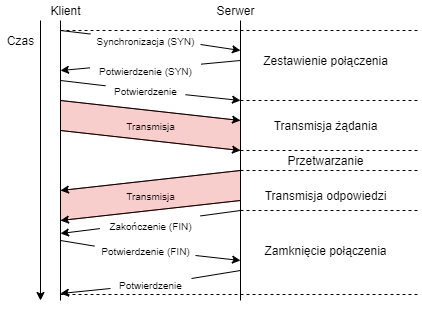
\includegraphics[width=90mm]{Rysunki/Rozdzial3/tcptransmission.png}
    \caption{TCP transmission diagram}
    \label{fig:my_label}
\end{figure}

TCP (\emph{Transmission Control Protocol}) is a connection oriented protocol, which means that at the start of the transmission, a session between the transmitter and the receiver is created. Additionally, it is characterized by reliability, due to the requirement of getting an acknowledgement for each transmitted packet, and performing a retransmission in case of transmission errors or lack of acknowledgement. This characteristics is especially important in case of exchanging data, which integrity plays a key role, such as files or e-mail messages. Primary protocols in the application layer which utilize TCP transmission are: HTTP, HTTPS, FTP, SMTP and Telnet \cite{tcpip:layers}. The flow of a singular transmission is presented on figure 3.1.

UDP (\emph{User Datagram Protocol}), on contrary to the TCP, is not a connection oriented protocol and it does not perform any retransmissions. This means that transmitting a message using the UDP protocol does not guarantee that it reach the recipient. Additionally, the order in which the packets are received does not need to reflect the order of their transmission, which requires sorting by the recipient devices. The advantage of UDP protocol however is increased speed of the transmission thanks to significant simplification of utilized mechanisms. This comes especially handy in case of services, where losing singular packets is not a problem, and keeping a low latency is of much bigger importance. This especially concerns voice transmission, and online video games. Example protocols utilizing UDP transmission are: DNS, DHCP, TFTP, SNMP, RIP and VOIP \cite{tcpip:layers}. The flow of singular transmission was presented on figure 3.2. 


\begin{figure}[!ht]
    \centering
    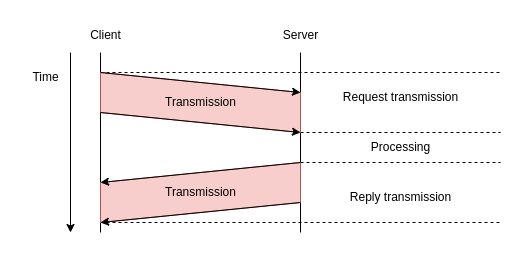
\includegraphics[width=100mm]{Rysunki/Rozdzial3/udptransmission.png}
    \caption{UDP transmission diagram}
    \label{fig:my_label}
\end{figure}

\section{Network layer}

In this layer, the transmission frame is wrapped in address fields containing the IP addresses of the sender and the recipient. Their presence is important due to the method of routing data in the Internet, which bases on passing the packet between subsequent devices until it reaches the recipient. Network devices know know on which port the packet should be forwarded thanks to their configuration. The IP protocol used for addressing is available in version IPv4 and IPv6, which differ in the length of the addresses, the manner of addressing networks and subnetworks, and translation of the addresses between public and private in case of IPv4, or lack thereof in case of IPv6.

Other than the IP protocol, the network layer offers following protocols:

\begin{itemize}
	\item [1)] ARP (\emph{Address Resolution Protocol}) -- it serves the purpose of acquiring the MAC address of the device with corresponding IP address;
	\item [2)] RARP (\emph{Reverse Address Resolution Protocol}) -- allows for acquiring the IP address of a device based on its MAC address;
	\item [3)] ICMP (\emph{Internet Control Message Protocol}) -- a protocol allowing to oversee the state of given computer network.
\end{itemize}

The necessity of use of protocols which give access to MAC addresses based on IP addresses arises from the difference in addressing between the network layer, which uses IP addresses, and network access layer, which uses MAC addresses. During the transmission of a packet, each of the intermediary devices performs packet decapsulation to the form available in network layer, and subsequently makes the decision whether the packet should be forwarded further based on the IP address. In case of the need to forward the message to another device, it is encapsulated again with information about MAC addresses in the network access layer. In the opposite case the packet is forwarded to the higher layers. Figure 3.3. shows the layer diagram, in which a packet is processed during transmission between two intermediary devices.  

\begin{figure}[!ht]
    \centering
    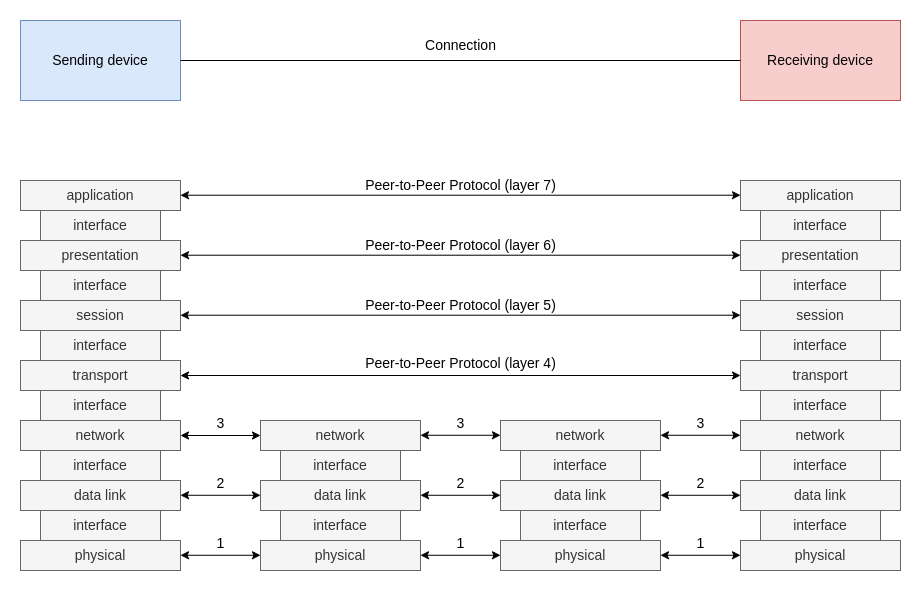
\includegraphics[width=155mm]{Rysunki/Rozdzial3/osi_route.png}
    \caption{Packet path diagram in the OSI model - Computer Notes}
    \label{fig:my_label}
\end{figure}

\section{Network access layer}

The layer responsible for preparing the packets for transmission using the physical medium, and carrying out the transmission. Both in case of wired and wireless networks, following sublayers can be identified:

\begin{itemize}
	\item [1)] LLC (\emph{Logic Link Control}) -- concatenates the frame with information about the protocol used in transport layer, in order to allow the recipient device to correctly interpret the received packet;
	\item [2)] MAC (\emph{Media Access Control}) -- creates the physical addresses sections in the Ethernet frame, storing MAC address of the sender and either the recipient, or intermediary router. In case of intermediary routers, the recipient address is updated by the router during the forwarding of the packet;
	\item [3)] PHY (\emph{Physical}) -- consists of elements of the physical medium for transmission, such as transmission wires, antennas and transceivers;
\end{itemize}

Two primary connectivity methods can be distinguished on the physical interface level: wired and wireless/

\subsection{Wired connectivity}

In order to connect devices in a wired manner, an UTP cable is commonly used, which utilizes the 8P8C connector, commonly incorrectly called RJ-45 due to very similar shape (RJ-45 connector has additional extrusion) \cite{8p8c}. The 8P8C is an 8-pin connector, which has 4 pairs of wires marked by straight and dashed isolation colors. It allows for connecting two devices via Point-to-Point method, using the PPPoE protocol (\emph{Point-to-Point Protocol over Ethernet}). This connector is often found both in form of extension modules which use serial interfaces, as in form of integrated port on the circuit board. Figure 3.4 presents the enumeration of 8P8C port lines, and figure 3.5 presents the enumeration for 8P8C connector.

\begin{figure}[!ht]
    \centering
    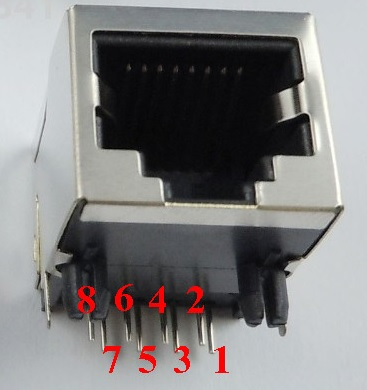
\includegraphics[width=30mm]{Rysunki/Rozdzial3/rj45 jack.jpg}
    \caption{8P8C port line enumeration - Electronics Stack Exchange}
    \label{fig:my_label}
\end{figure}

\begin{figure}[!ht]
    \centering
    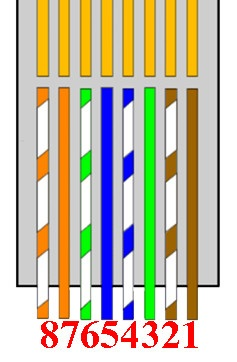
\includegraphics[width=25mm]{Rysunki/Rozdzial3/rj45 plug.jpg}
    \caption{8P8C connector line enumeration - Electronics Stack Exchange}
    \label{fig:my_label}
\end{figure}

The connection between the MAC and the PHY layers is carried out via platform-independent MII interface (\emph{Media-Independent Interface}) or its reduced version RMII (\emph{Reduced Media-Independent Interface}). It takes form of a connection between the processing unit and the Ethernet port driver, equipped with DAC (\emph{Digital-Analog Converter}) and ADC (\emph{Analog-Digital Converter}) in order to allow for transmission via differential signal through the Ethernet cable. Figure 3.6 presents a functional diagram of a sample Ethernet driver, and figure 3.7 its placement in a platform blueprint between MAC and PHY layers.

\begin{figure}[!ht]
    \centering
    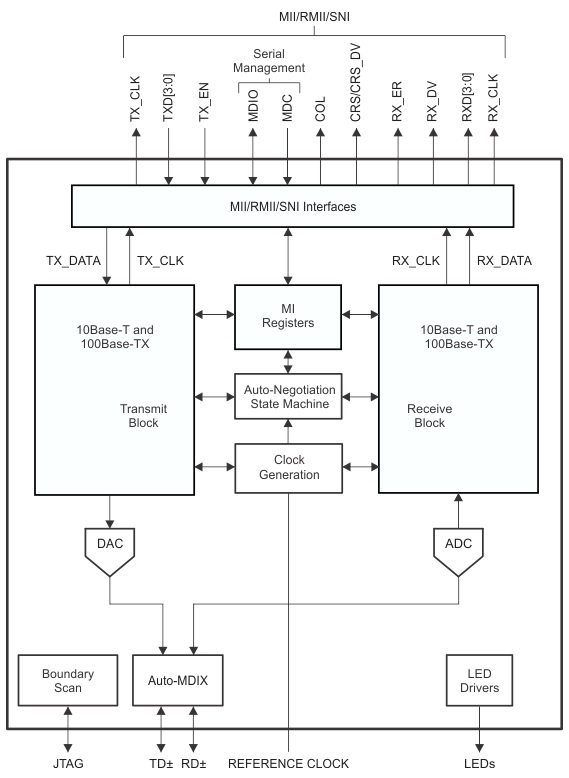
\includegraphics[width=70mm]{Rysunki/Rozdzial3/sterownik-rj45.jpg}
    \caption{Functional diagram of DB83848-P Ethernet driver by Texas Instruments - Texas Instruments}
    \label{fig:my_label}
\end{figure}

\begin{figure}[!ht]
    \centering
    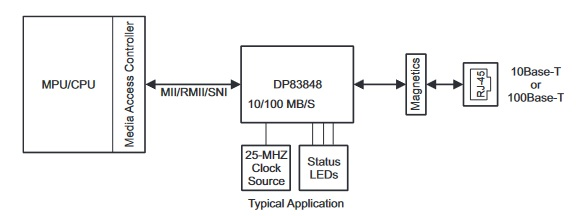
\includegraphics[width=80mm]{Rysunki/Rozdzial3/driverplacement.jpg}
    \caption{DB83848-P driver placement - Texas Instruments}
    \label{fig:my_label}
\end{figure}

The use of RMII allows for connecting different physical mediums (such as UTP cable, fibre optics) to the same data link layer. Table 3.1 describes the lines present in the RMII and their purposes \cite{wiki:rmii}\cite{artykul:rmii}. The MAC abbreviation stands for data link layer, and the PHY abbreviation stands for physical layer.

\begin{table}[!ht]
    \centering
    \caption{RMII lines}
    \begin{tabular}{c|c|c}
        Line designation & Transmission direction & Description  \\
        \hline
        REF\texttt{\char`_}CLK & Any one-way & Reference clock 50 MHz \\
        TXD0 & MAC -> PHY & First transmission bit \\
        TXD1 & MAC -> PHY & Second transmission bit \\
        TX\texttt{\char`_}EN & MAC -> PHY & Transmission start signal \\
        RXD0 & PHY -> MAC & First reception bit \\
        RXD1 & PHY -> MAC & Second reception bit \\
        CRS\texttt{\char`_}DV & PHY -> MAC & Carrier detection line \\
        RX\texttt{\char`_}ER & PHY -> MAC & Reception error line \\
        MDIO & two-way & Administrative data line \\
        MDC & MAC -> PHY & Clock signal for line MDIO
    \end{tabular}
    \label{tab:my_label}
\end{table}

Transmitting via RMII requires converting the binary representation of the code of sent character to big-endian notation, which even index bits (starting enumerating from 0) are transmitted via line TXD0, and odd index bits via line TXD1, creating so called \emph{di-bit} or \emph{nibble} transmission. Similarly to the transmission, reception of the data happens by receiving bits with even index (with enumerating from 0) on line RXD0 and bits with odd indexes on line RXD1.

The connection of lines within the UTP cables for the 8P8C connectors is an important matter. In case of connecting two devices deemed as \emph{hosts}, it is necessary to use a crossover cable, which is a cable where the transmitting and receiving pair between each end of the cable are switched. However in case of connecting a host to a device such as a router (which has an on-board switch), a straight-thru cable needs to be used. Those two ways of making the 8P8C connector for the UTP cable are known as T-568A and T-568B respectively.

\begin{figure}[!ht]
    \centering
    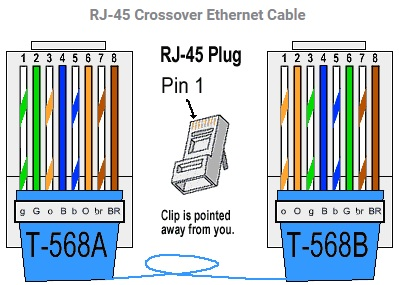
\includegraphics[width=54mm]{Rysunki/Rozdzial3/cross.jpg}
    \caption{Line placement in UTP cable - The Internet Centre Inc.}
    \label{fig:my_label}
\end{figure}

\newpage
\subsection{Wireless connectivity}

Thanks to the popularity of integration of embedded systems with wireless networks, especially in case of home and office automation, the market offers a number of different modules providing wireless network functionalities, both for Wi-Fi and cellular data. Due to their very similar construction, in which the major difference often is only the type of antenna for given frequency, this thesis provides only a general description of said modules.

Majority of the modules are available in the form of preprogrammed digital circuits on a PCB board, most commonly with integrated mocroband antenna (in form of a path on the printed board), with SMA antenna port used for concentric cables, IPEX port, or u.FL port. Figure 3.7 presents example antennas used by wireless modules.

\begin{figure}[!ht]
    \centering
    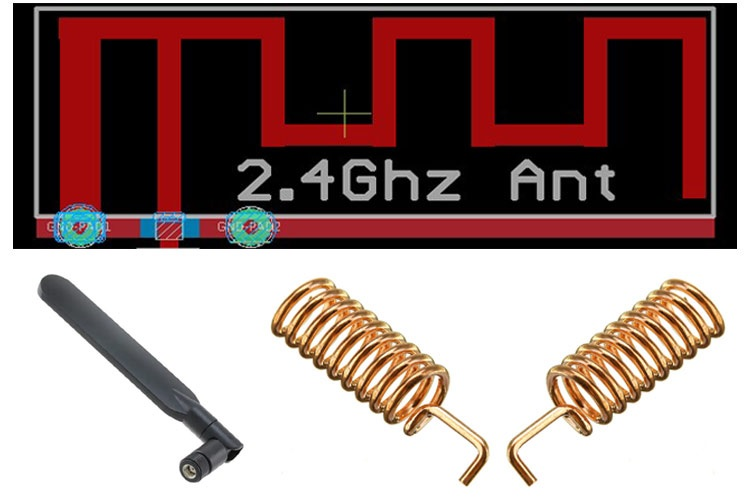
\includegraphics[width=45mm]{Rysunki/Rozdzial3/antenna.jpg}
    \caption{Antenna types for embedded systems - Circuit Digest}
    \label{fig:my_label}
\end{figure}

Part of the circuits which implement the wireless interface are available in a form of a Shield extension, which allows for very easy integration with Arduino hardware platform, without the need for soldering. The construction of such module is very similar to the Arduino hardware platform itself, having ports that are corresponding with function and placement to the ones present on the microcontroller board. In case of modules which offer the GSM connectivity, it is necessary to additionally provide a SIM card, similarly to the common mobile phones.

\begin{figure}[!ht]
\begin{minipage}[b]{0.4\textwidth}
    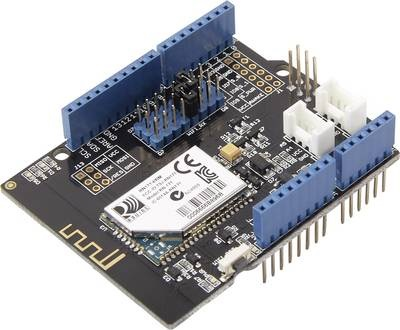
\includegraphics[width=60mm]{Rysunki/Rozdzial3/shield.jpg}
    \caption{Wi-Fi Shield - Seeed Studio}
  \end{minipage}
  \hfill
  \begin{minipage}[b]{0.4\textwidth}
    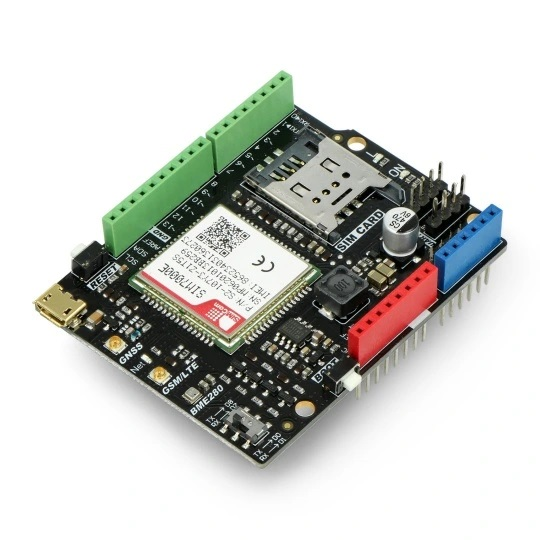
\includegraphics[width=60mm]{Rysunki/Rozdzial3/gsm.jpg}
    \caption{GSM Shield - Botland}
  \end{minipage}
\end{figure}

\newpage
\section{TCP/IP stack implementation}

Implementation of TCP/IP stack, both due to the number and the complexity of the protocols, is a complex task. Because of that, the most common approach is to use already established solutions. Some of the devices (especially extension modules) implement the whole TCP/IP stack, requiring from the user only implementing the communication with selected local serial interface, such as SPI or I$^2$C.

\begin{figure}[!ht]
    \centering
    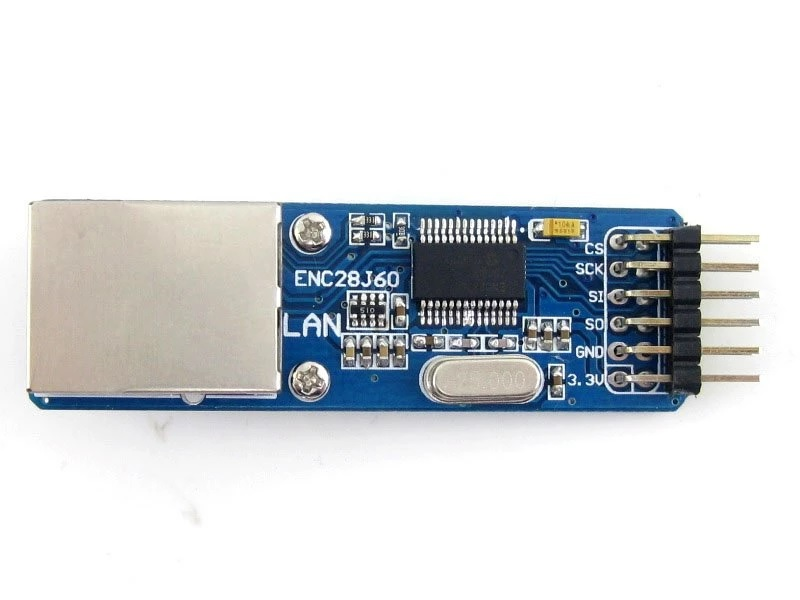
\includegraphics[width=60mm]{Rysunki/Rozdzial3/enc28j60.jpg}
    \caption{ENC28J60 module - Aliexpress}
    \label{fig:my_label}
\end{figure}

ENC28J60 module \cite{enc28j60} is an example of solution providing an external Ethernet interface, which was shown on figure 3.12. It has compatibility with 10/100/1000Base-T networks, supporting especially 10Base-T transmission. In order to communicate with a microcontroller, and SPI interface with the clock frequency of 20 MHz is used. It provides only the implementation of physical and data link layer of the OSI model, which forces the user to implement the other layers of the TCP/IP stack on their own. Said module possesses an 8kB programmable memory for reception and transmission buffers and hardware control sum calculation. Thanks to implementing the application layer on the microcontroller, the amount of available network logical sockets is entirely dependent on the RAM memory size of the microcontroller.

\begin{figure}[!ht]
    \centering
    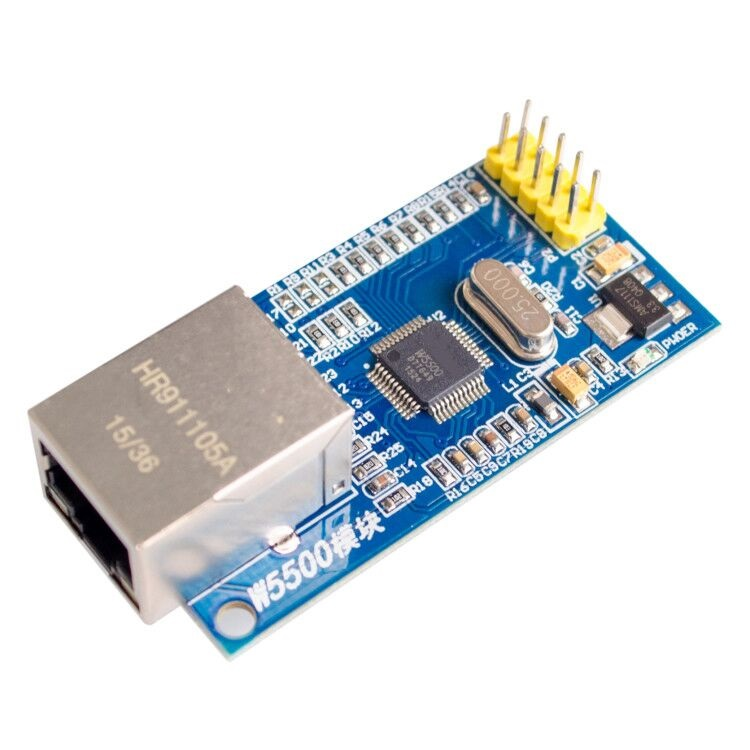
\includegraphics[width=60mm]{Rysunki/Rozdzial3/w5500.jpg}
    \caption{W5500 module - Aliexpress}
    \label{fig:my_label}
\end{figure}

W5500 is another example of wired connectivity as shown on figure 3.13. On contrary to the ENC28J60 module, it offers also part of the higher layers protocols, such as TCP, UDP, ICMP, IPv4, ARP, IGMP and PPPoE \cite{w5500}. Additionally it provides the functionality of \emph{wake on LAN}. This module is also available in the form of Shield extension for the Arduino boards. It operates with standards 10/100 Base-T and contains 32 kB programmable memory for transmission and reception buffers, and supports 8 logical network sockets. The module operates with 3.3 V power level, while tolerating 5 V on the I/O (Input/Output) pins. Table 3.2 presents the comparison of aforementioned modules with reference prices. 

\begin{table}[!ht]
    \centering
    \caption{Ethernet module parameters comparison}
    \begin{tabular}{c|c|c|c|c|c}
        \multirow{2}{*}{Module} & Standard & \multirow{2}{*}{Protocols} & \multirow{2}{*}{Interface} & Speed & \multirow{2}{*}{Price} \\
        & Transmission & & & Interface \\
        \hline
        ENC28J60 & 10Base-T & MAC & SPI & 20 MHz & 32.70 PLN \\
        \hline
        \multirow{3}{*}{W5500} & \multirow{3}{*}{10/100Base-T} & MAC, TCP, UDP, & \multirow{3}{*}{SPI} & \multirow{3}{*}{80 MHz} & \multirow{3}{*}{115.00 PLN} \\
        & & ICMP, IPv4, ARP, & & & \\
        & & & IGMP, PPPoE & &
    \end{tabular}
    \label{tab:my_label}
\end{table}

Two of the most popular wireless connectivity modules are ESP8266 and ESP32, presented by figures 3.14 and 3.15 respectively. The later module is a newer version of the former one. Both of the modules operate in 2.4 GHz band, with the IEEE 802.11 b/g/n standards. They differ in available speeds, security features and serial interfaces providing connection with the microcontroller. Both modules use pad and THT connectors, allowing the user to solder in the goldpin pins. Both ESP8266 and ESP32 can operate in the softAP (\emph{Soft Access Point}) mode and as a transceiving station (\emph{STA}).

\begin{figure}[!ht]
\begin{minipage}[b]{0.4\textwidth}
    \centering
    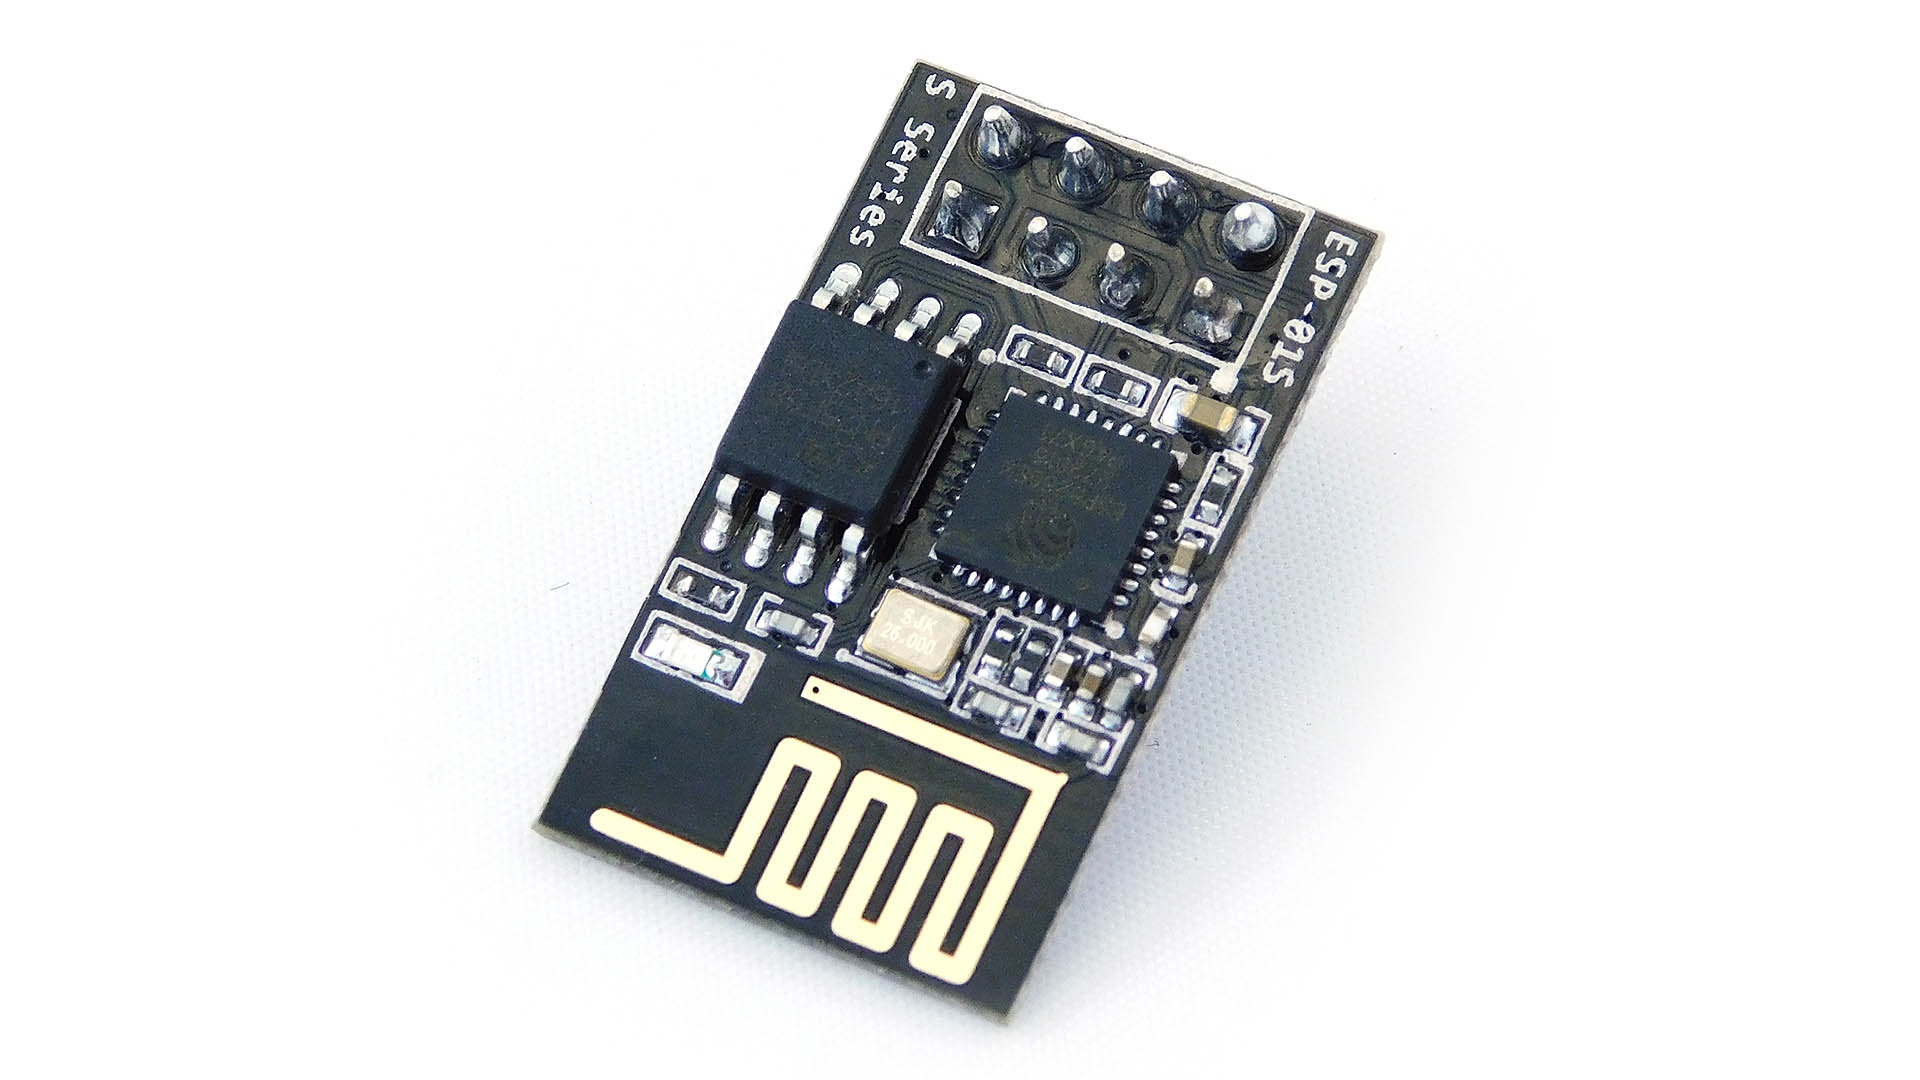
\includegraphics[width=70mm]{Rysunki/Rozdzial3/esp8266.jpg}
    \caption{ESP8266 module - Nettigo}
  \end{minipage}
  \hfill
  \begin{minipage}[b]{0.4\textwidth}
    \centering
    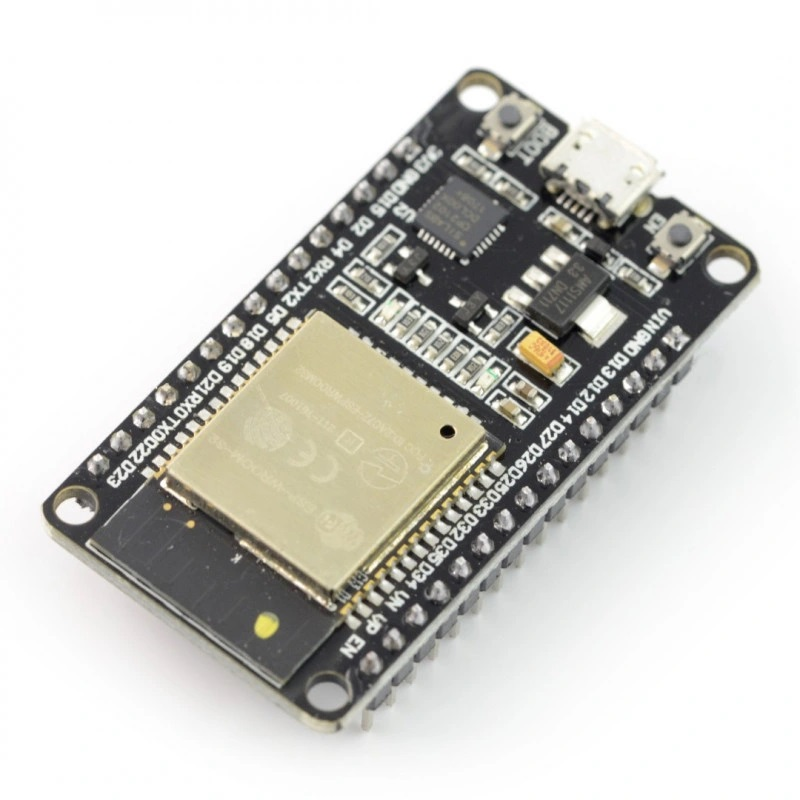
\includegraphics[width=40mm]{Rysunki/Rozdzial3/esp32.jpg}
    \caption{ESP32 module - Botland}
  \end{minipage}
\end{figure}

ESP8266 provides the communication speed up to 72.2 Mbps. \emph{Firmware} delivered by the module manufacturer implements IPv4, TCP, UDP, HTTP, ICMP and MAC protocols and offers encryption via WEP, WPA/WPA2, TKIP and AES algorithms \cite{esp8266}. In order to communicate with microcontroller, it uses the UART (\emph{Universal Asynchronous Receiver Transmitter}) interface, and uses AT commands in order to control the module. Its operating voltage is around 3.3 V, and two antenna types are available - a microband integrated antenna, or an u.FL port.

ESP32 is a newer version or said ESP8266. The circuit contains a dual core processing unit, which allowed for increasing the transmission speed up to 150 Mbps \cite{esp32}. Similarly to ESP8266, the manufacturer provides \emph{firmware} which implements IPv4, TCP, UDP, HTTP, ICMP and MAC protocols, but has more extensive security features, extending the encryption algorithm range by PSK/Enterprise, SHA-2, ECC and RSA-4096 algorithms. Some of the variants of the module have integrated support for IPv6 protocol. There is a possibility for the user to create their custom version of said firmware, containing protocols suited for their needs, using the SDK (\emph{Software Development Kit}) provided by the manufacturer. The module operates with the voltage of 3.3 V. In order to communicate with the microcontroller, user can use either SPI, I$^2$C or UART interfaces. Table 3.3 shows the comparison of the parameters of the modules along with their reference prices.

\begin{table}[!ht]
    \centering
    \caption{Overview of wireless modules parameters}
    \begin{tabular}{c|c|c|c|c|c}
        \multirow{2}{*}{Module} & Standard & \multirow{2}{*}{Protocol} & \multirow{2}{*}{Interface} & Speed & \multirow{2}{*}{Price} \\
        & of transmission & & & of transmission \\
        \hline
        \multirow{2}{*}{ESP8266} & \multirow{2}{*}{802.11 b/g/n} & MAC, TCP, UDP, & \multirow{2}{*}{UART} & \multirow{2}{*}{72,2 Mbps} & \multirow{2}{*}{14.90 PLN} \\
                & & HTTP, IPv4, ICMP & & & \\
        \hline
        \multirow{3}{*}{ESP32} & \multirow{3}{*}{802.11 b/g/n} & MAC, TCP, UDP, & \multirow{2}{*}{SPI, I$^2$C,} & \multirow{3}{*}{150 Mbps} & \multirow{3}{*}{127.50 PLN} \\
        & & HTTP, IPv4, (IPv6), & \multirow{2}{*}{UART} & & \\
        & & ICMP & & &
    \end{tabular}
    \label{tab:my_label}
\end{table}

\begin{figure}[!ht]
    \centering
    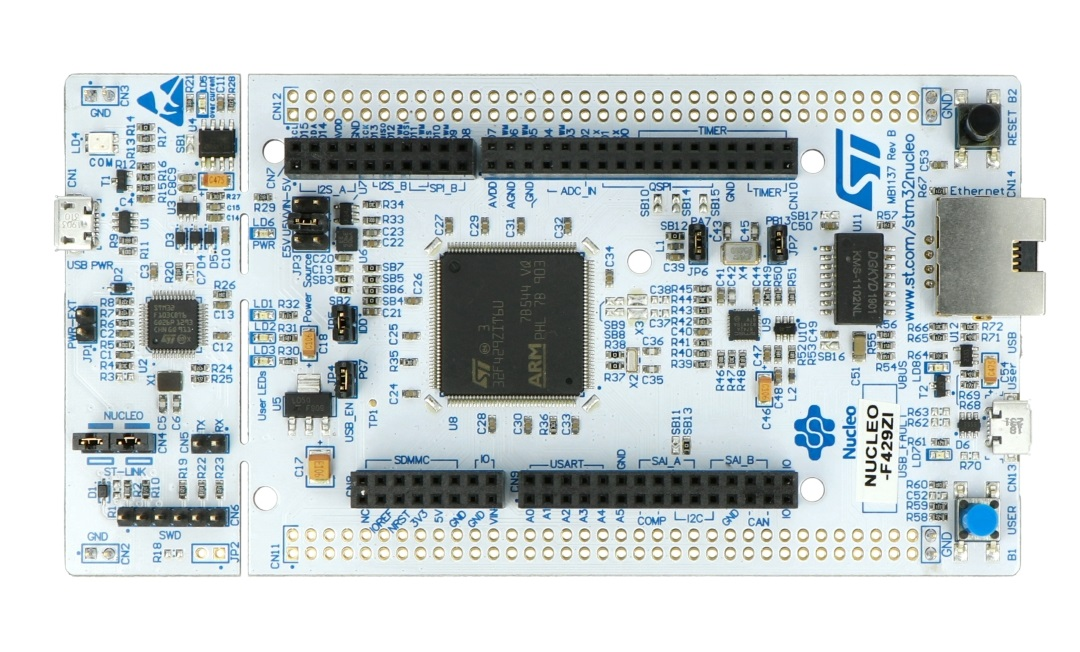
\includegraphics[width=100mm]{Rysunki/Rozdzial3/nucleo.jpg}
    \caption{Nucleo-F429ZI platform with integrated Ethernet port \dywiz{} Botland}
    \label{fig:my_label}
\end{figure}

Some of the manufacturers of hardware platform decide to partially implement the TCP/IP stack for their platforms in cases, when they are equipped with integrated network interface (such as 8P8C port). Nucleo-F4 are a good example of such platforms (eg. Nucleo-F429ZI board shown by figure 3.16) equipped with integrated 8P8C port. The HAL (\emph{Hardware Abstract Layer}) software distributed by the ST Microelectronics for said microcontrollers provides the implementation of the network access layer, however it does not offer the higher layers, requiring the user to utilize middleware, such as eg. open source LwIP (\emph{Lightweight IP}) or uIP (\emph{micro IP}) stacks. In order to use the said protocol stacks, they need to be ported first for given microcontroller, or the user needs to use an already available solution if it has been created so far.

The LwIP stack contains the implementation of protocols of application, transport and network layer. Those protocols are as follows \cite{lwip:protocols}:

\begin{itemize}
    \item [1)] IP;
    \item [2)] ICMP;
    \item [3)] UDP;
    \item [4)] DHCP;
    \item [5)] TCP;
    \item [6)] ARP;
    \item [7)] BSD (optionally)
\end{itemize}

Since version v.2.0.0 the LwIP stack supports both IPv4 and IPv6 addressing. 

uIP is an open-source implementation of the TCP/IP stack dedicated for microcontrollers with very limited Flash and RAM memory. According to the document \cite{ti:uip} the uIP stack can minimize the RAM usage to a couple hundred bytes. It implements the following protocols:

\begin{itemize}
    \item [1)] TCP;
    \item [2)] UDP;
    \item [3)] IP;
    \item [4)] ICMP;
    \item [5)] ARP
\end{itemize}

Due to very harsh requirements regarding memory optimization, all application layer protocols are left for implementation by the user. This decision was also made in part due to being unable to predict what specific applications the stack will be used for.
\chapter{Practical implementation of the network interface}
%=================================================================================================
\section{Project goals}

Following project goals were defined while constructing the practical solution: 

\begin{itemize}
    \item [1)] The implementation will consist of a wired network interface using Ethernet and wireless network interface using ESP8266 module;
    \item [2)] The IoT module will receive the network information such as its assigned IP address, subnetwork mask and gateway IP via DHCP service;
    \item [3)] Solution will allow to establish communication with the device using the \emph{ping} command;
    \item [4)] Solution will offer an echo server which will relay back messages received by the IoT module via TCP protocol back to the sender.
\end{itemize}

%=================================================================================================
\section{Chosen components}
\subsection{Hardware platform}

Due to the already available physical implementation for 8P8C socket and wide availability of reference materials such as documentation and resources produced by the community, Nucleo-F429ZI by ST Microelectronics was chosen as the target hardware platform. In order to implement the wireless interface, the aforementioned ESP8266 module was used due to its small cost.

\subsection{Environment and programming language}

During the analysis of available resources a decision was undertaken to pick STM32\dywiz CubeIDE which is the dedicated environment for the chosen hardware platform, as the IDE of choice. This is a result of the availability of embedded configuration tools, which allow for configuring selected parameters of the hardware platform without the need to manually manipulate the registers of the microcontroller. The programming language was determined to be C.

\subsection{Verification methods of the system functionality}

Verification of the system functionality will happen in a two-step process. First step includes transferring information about the IoT module, such as its IP address, subnetwork mask and gateway address via a virtual serial port. Second step consists of an attempt to communicate with the module via \emph{ping} command and communication with the implemented echo server using Hercules SETUP Utility software, which allows communication using the TCP protocol. 

%=================================================================================================
\section{Hardware implementation}

\subsection{Ethernet interface}

Thanks to the selected hardware platform, the hardware implementation was already done in-factory on the Nucleo-F429ZI board. The board contains soldered in 8P8C connector with designated RMII interface, as presented on figure 4.1.

\begin{figure}[!ht]
    \centering
    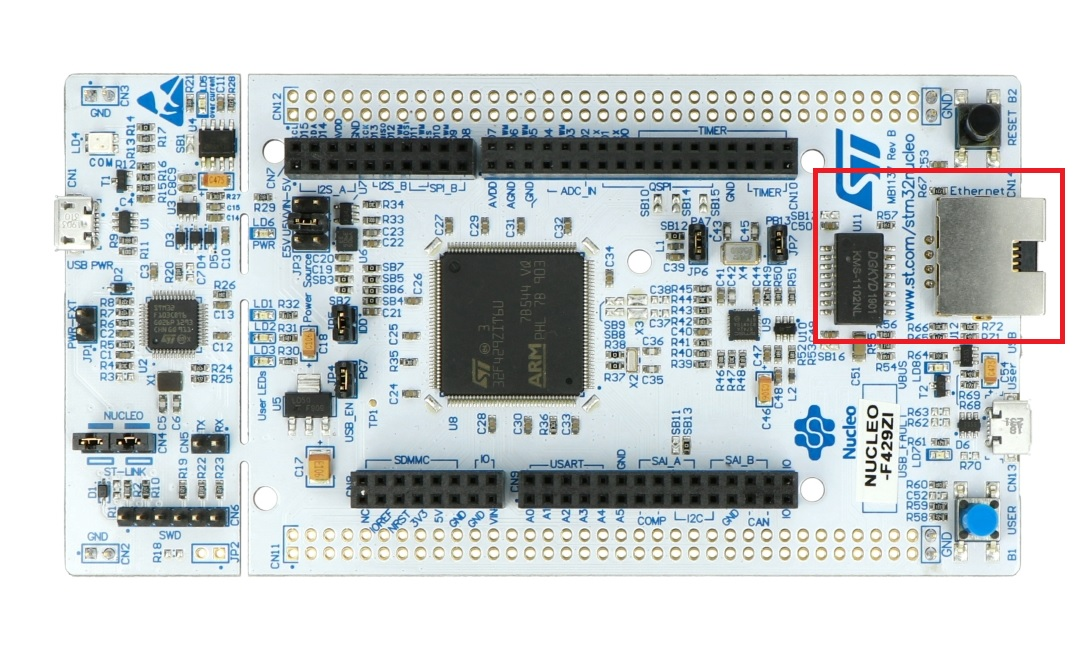
\includegraphics[width=120mm]{Rysunki/Rozdzial4/nucleo 8p8c.jpg}
    \caption{8P8C connector present on the Nucleo-F429ZI board}
    \label{fig:my_label}
\end{figure}

\subsection{Wireless interface}

In order to communicate with the ESP8266 module, an USART6 serial interface of the STM32-F429ZI microcontroller was used. It is present at pins PC6 and PC7. Additionally a PB3 pin was used in order to provide logical high level to the \emph{enable} input pin of the ESP8266. Figure 4.2 shows the schematic of the connections.

\begin{figure}[!ht]
    \centering
    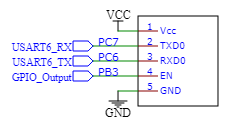
\includegraphics{Rysunki/Rozdzial4/schemat_esp8266.png}
    \caption{ESP8266 connection schematic}
    \label{fig:my_label}
\end{figure}

%=================================================================================================
\section{Software implementation}

\subsection{Ethernet interface}

The first step of the implementation consisted of initializing the Ethernet interface allowing for correct transmission of the \emph{ping} packet and to signalize the state of the connection via an LED.

Initialization process started by launching the STM32CubeIDE environment and creating a new project selecting STM32L429ZI microcontroller. Figure 4.3 shows the microcontroller platform selection, and figure 4.4 options of the created project.

\begin{figure}[!ht]
    \centering
    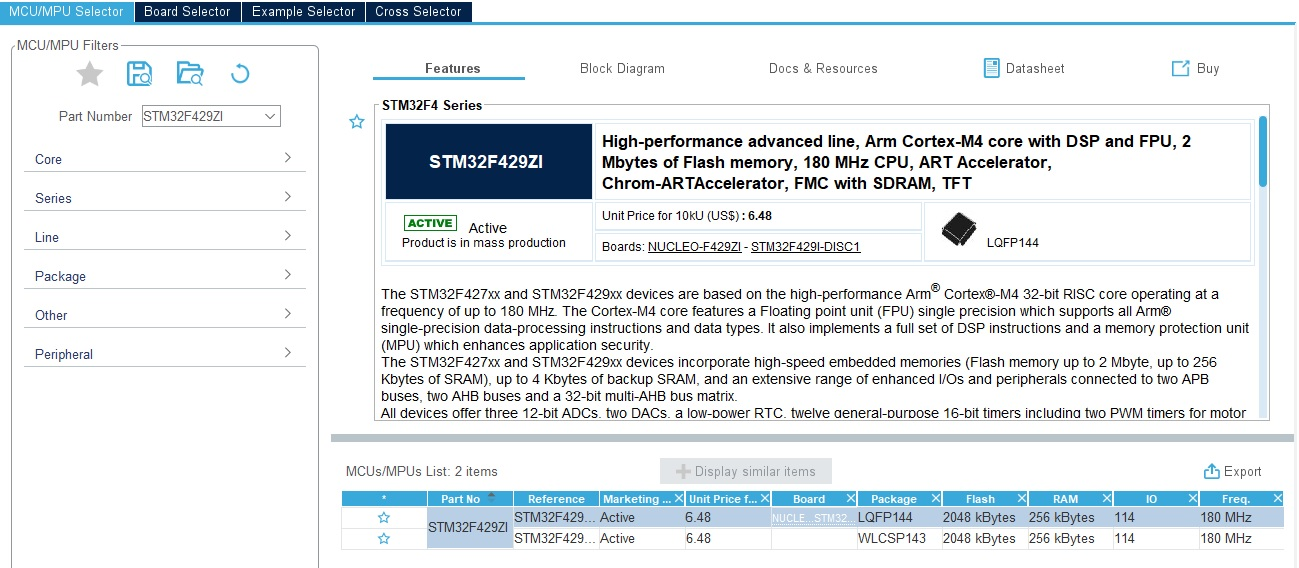
\includegraphics[width=155mm]{Rysunki/Rozdzial4/wybór mikrokontrolera.jpg}
    \caption{Microcontroller selection in STM32CubeIDE}
    \label{fig:my_label}
\end{figure}

\begin{figure}[!ht]
    \centering
    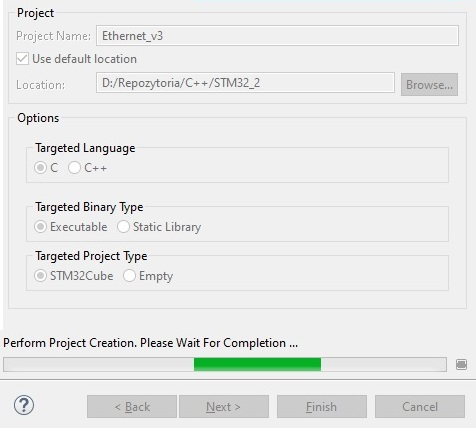
\includegraphics[width=80mm]{Rysunki/Rozdzial4/utworzenie projektu.jpg}
    \caption{Creating the project}
    \label{fig:my_label}
\end{figure}

\newpage
The clock signal provided by ST-LINK module being an embedded part of the Nucleo-F429ZI board was used as the system clock. In order to achieve this, High Speed Clock in the RRC tab needed to be set to BYPASS, which was showcased by the figure 4.5. Resulting configuration of the clocking signal was presented on figure 4.6.

\begin{figure}[!ht]
    \centering
    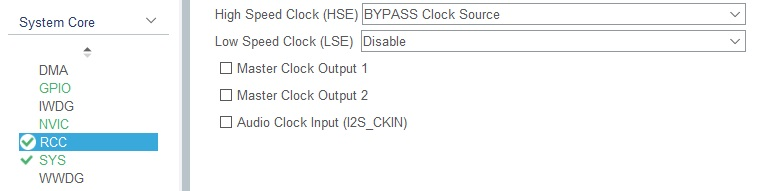
\includegraphics[width=120mm]{Rysunki/Rozdzial4/tryb bypass.jpg}
    \caption{Switching the HSE clock into BYPASS mode}
    \label{fig:my_label}
\end{figure}

\begin{figure}[!ht]
    \centering
    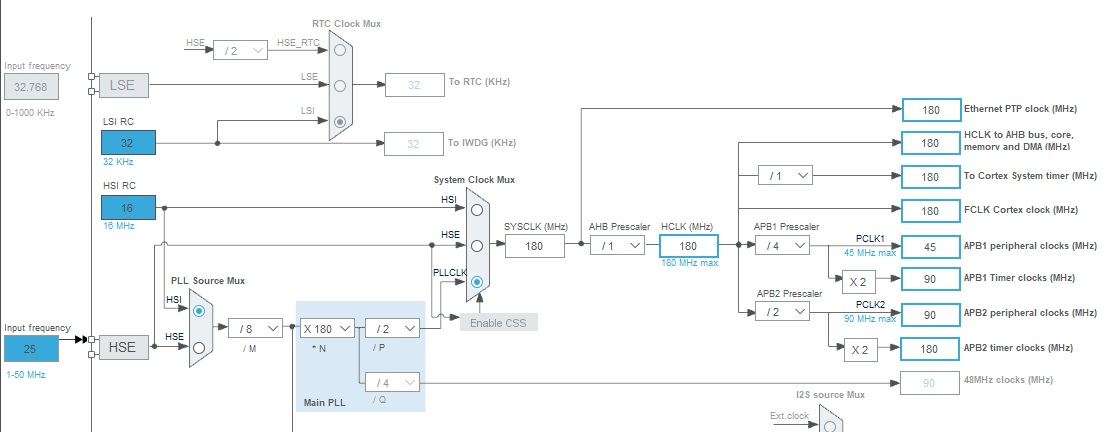
\includegraphics[width=155mm]{Rysunki/Rozdzial4/clock_signal_bypass.jpg}
    \caption{Configuring clocking signal after switching HSE to BYPASS mode}
    \label{fig:my_label}
\end{figure}

\newpage
The Ethernet interface needs to be initially configured in the \emph{Connectivity} tab, setting its mode to RMII. It is a result of the Nucleo-429ZI board structure, in which the Ethernet connection is realized using RMII interface. The default MAC address of the device is equal to 00:80:E1:00:00:00. During the setup of default values via a configurator, the PHY address of the device was assigned as 1. It needed to be changed to 0. The results were shown on figures 4.7 and 4.8.


\begin{figure}[!ht]
    \centering
    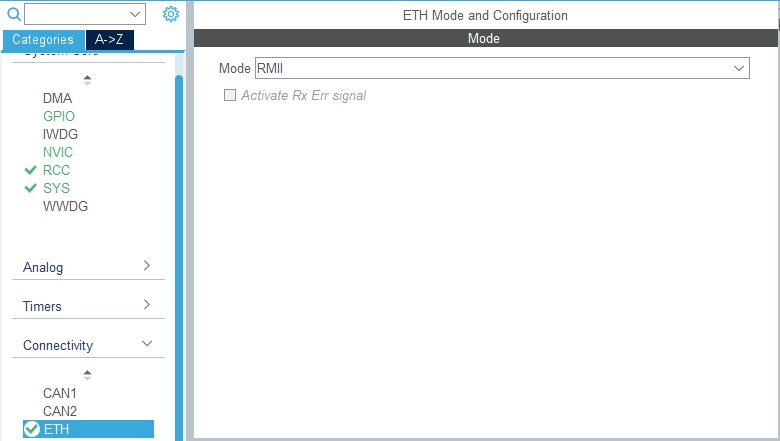
\includegraphics[width=120mm]{Rysunki/Rozdzial4/rmii1.jpg}
    \caption{Assigning RMII mode to the Ethernet interface}
    \label{fig:my_label}
\end{figure}

\begin{figure}[!ht]
    \centering
    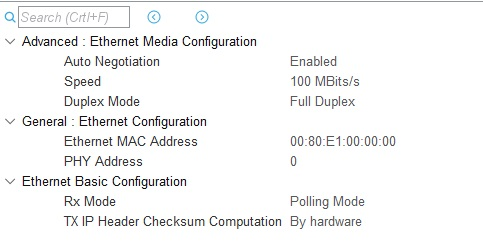
\includegraphics[width=120mm]{Rysunki/Rozdzial4/rmii2.jpg}
    \caption{Target values of RMII parameters}
    \label{fig:my_label}
\end{figure}

Due to the connections present on the Nucleo-F429ZI board in accordance to the table presented in the manufacturer documentation \cite{nucleo-manual} the output pins of the microcontroller were assigned in a way showcased in table 4.1. The RMII interface connection schematics are presented by figure 4.9.

\newpage

\begin{figure}[!ht]
    \centering
    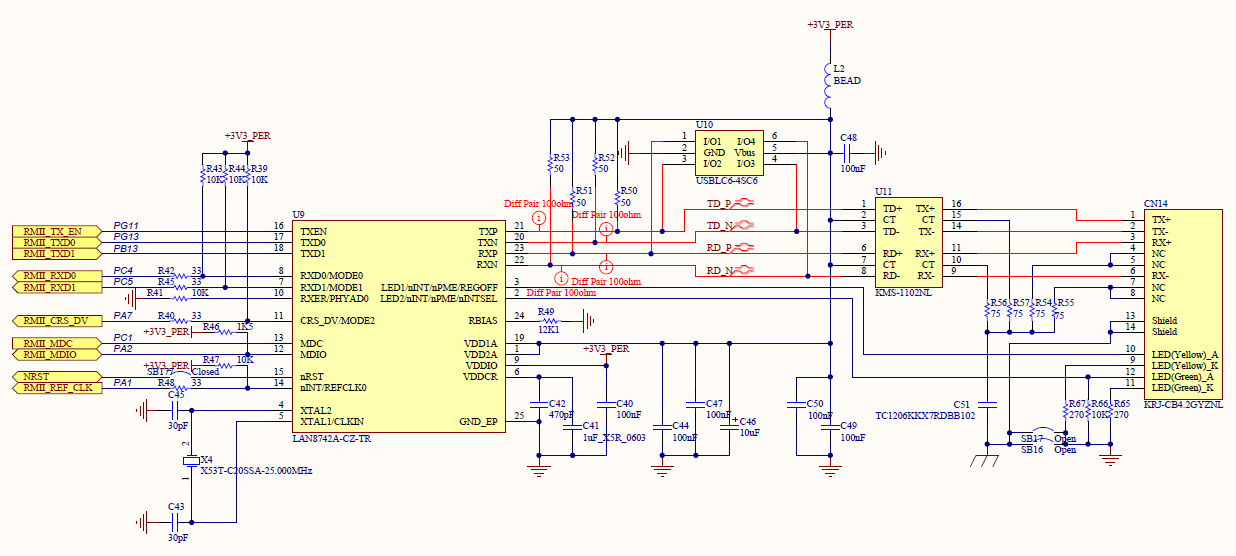
\includegraphics[width=140mm]{Rysunki/Rozdzial4/schemat_RMII.png}
    \caption{RMII interface connection schematics}
    \label{fig:my_label}
\end{figure}

{\centering

\begin{longtable}{c|c}
    \caption{Output line assignment} \\
    Pin name & Functionality \\
    \hline
    PA1 & ETH\texttt{\char`_}REF\texttt{\char`_}CLK \\
    PA2 & ETH\texttt{\char`_}MDIO \\
    PA7 & ETH\texttt{\char`_}CRS\texttt{\char`_}DV \\
    PC4 & ETH\texttt{\char`_}RXD0 \\
    PC5 & ETH\texttt{\char`_}RXD1 \\
    PG11 & ETH\texttt{\char`_}TX\texttt{\char`_}EN \\
    PG13 & ETH\texttt{\char`_}TXD0 \\
    PB13 & ETH\texttt{\char`_}TXD1 \\
    PB14 & Red LED \\
    PB0 & Green LED \\
    PB7 & Blue LED \\
    Pin name & Functionality \\
    \hline
    PD9 & RX line of virtual serial port USART3 \\
    PD8 & TX line of virtual serial port USART3
    \label{tab:my_label}
\end{longtable}
}

The next step included configuring the LwIP stacked used for operating the TCP/IP stack protocols. In order to do that, user needs to proceed to the \emph{Middleware} tab as shown on figure 4.10, where the user gains access to various software for selected microcontroller, such as the LwIP stack or freeRTOS real time operating system. The LwIP stack is characterized by big selection of configuration options. In the implementation for the needs of this dissertation, majority of the configuration can be left as default. User needs to make sure however that the LWIP\texttt{\char`_}NETIF\texttt{\char`_}LINK\texttt{\char`_}CALL-BACK, which designates a function called when the Ethernet connector is plugged in to 8P8C socket, is enabled, as shown on figure 4.11. 

\begin{figure}[!ht]
    \centering
    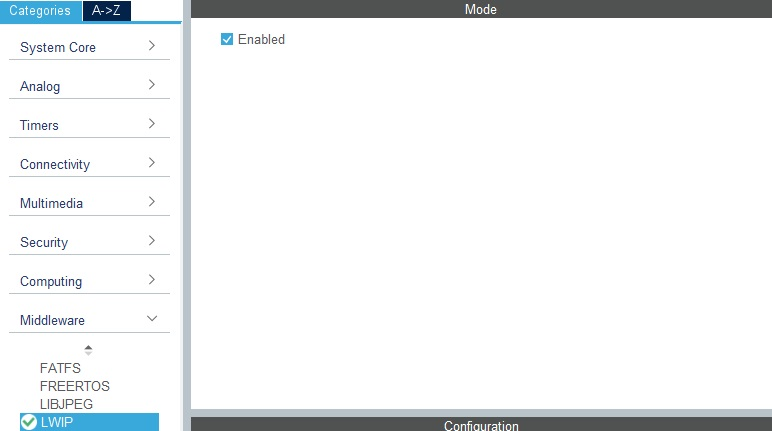
\includegraphics[width=120mm]{Rysunki/Rozdzial4/middleware_lwip.jpg}
    \caption{Enabling LwIP stack}
    \label{fig:my_label}
\end{figure}

\begin{figure}[!ht]
    \centering
    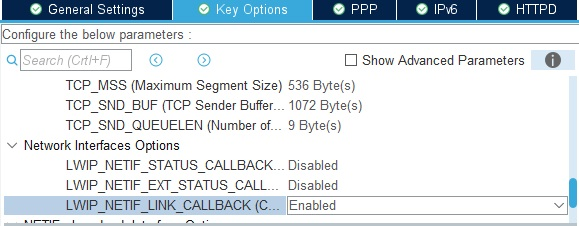
\includegraphics[width=100mm]{Rysunki/Rozdzial4/middleware_lwip_2.jpg}
    \caption{LWIP\texttt{\char`_}NETIF\texttt{\char`_}LINK\texttt{\char`_}CALLBACK option}
    \label{fig:my_label}
\end{figure}

\newpage
Using the \emph{Clock Configuration} tab, the Ethernet clock signal was set to the frequency of 180 MHz, via the PLL loop and correct prescalers, as presented by figure 4.12.

\begin{figure}[!ht]
    \centering
    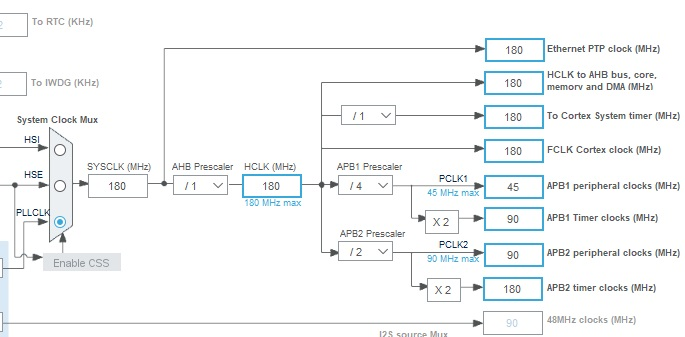
\includegraphics[width=120mm]{Rysunki/Rozdzial4/clock_config.jpg}
    \caption{Clock configuration}
    \label{fig:my_label}
\end{figure}

The follow up included generating the code and its modification. During the implementation of the echo server using the LwIP stack and modification of the \textit{MX\char`_LWIP\char`_Process()} function, it was decided to use a sample implementation by a korean Naver blog user nicknamed eziya76 \cite{eziya76}.

\cppcode{Listingi/Ethernet_main.c}{Ethernet implementation \textit{main()} function}

Listing 4.1 presents the contents of the \textit{main()} function for the project implementing the Ethernet interface. Part of this function was generated via the code generator based on the STM32CubeIDE environment configuration.

In order to store and format information regarding the connection, such as the IP address, subnetwork mask, gateway address, MAC address and connection status, 5 globally available buffers were created. This information is transmitted to the overseeing computer via USART3 serial port inside the \textit{notify\char`_dhcp\char`_status()} function.

The \textit{MX\char`_LWIP\char`_Process()} function takes care of receiving the dynamic IP address from the DHCP server enabled in the router and was presented on listing 4.2. The echo server is initialized in the \textit{init\char`_echo()}, repeating a copy of received message to the sender. Listing 4.3 showcases implementation of the \textit{notify\char`_dhcp\char`_status()} function. Listings 4.4 - 4.7 picture the implementation of functions that process information about connection and MAC address into a character string.

\cppcode{Listingi/LWIP_Process.c}{MX\textit{\char`_}LWIP\textit{\char`_}Process() function}

\newpage
\cppcode{Listingi/notify_dhcp_status.c}{Connection state overseeing function}

\cppcode{Listingi/parse_ip.c}{Function processing the IP address}

\cppcode{Listingi/parse_mask.c}{Function processing the subnetwork mask}

\cppcode{Listingi/parse_gateway.c}{Function processing the gateway address}

\newpage
\cppcode{Listingi/send_mac_address.c}{Function transferring the MAC address during the start of the device}

In order to control the echo server, a \textit{echo\char`_info} structure was created, which stores information regarding the connection status, retransmission count, pointer to the pcb structure of the LwIP stack and a pointer to the transceiveing buffer. Additionally, an enumerating type was created which allows to use connection state names instead of numerical values. Aforementioned elements were placed in a header file listed on listing 4.8. 

\cppcode{Listingi/echo.h}{Echo server header file}

The source file associated with the above header file contains prototypes and implementations of the callback functions, send function and connection shutdown function. They were presented on listing 4.9.

\cppcode{Listingi/echo.c}{A fragment of the echo server source file}

Starting the echo server begins with its initialization via the \textit{init\char`_echo()} function, called in the \textit{main()} function before the main loop. It creates a new TCP server object, connects it to a selected port and registers a connection accept callback. Port 7 was selected for the communication purposes. Listing 4.10. contains the code of the \textit{init\char`_echo()} function.

\cppcode{Listingi/init_echo.c}{TCP echo server initialization function}

The \textit{app\char`_callback\char`_accepted()} function is called when the connection is accepted by the server. It sets the priority of the created pcb, allocates the \textit{echo\char`_info} structure, sets its initial parameters and registers callbacks for data reception, error and polling. The code of those functions was placed on listing 4.11.

\cppcode{Listingi/app_callback_accepted.c}{Connection accept callback}

The next callback is \textit{app\char`_callback\char`_received()}, called during the data reception from the connected device. It takes care of supervising the buffers, engages sending data back to the sender in the form of echo, and accordingly modifies the connection state saved in the \textit{echo\char`_info} structure. Additionally it registers the \textit{app\char`_callback\char`_sent()} callback. Its code is presented by listing 4.12.

\cppcode{Listingi/app_callback_received.c}{Data reception callback function}

Function \textit{app\char`_callback\char`_sent()} oversees the situation after executing transmission. In case of subsequent data present, it initializes another transmission. \textit{app\char`_callback\char`_poll} function operates in a similar fashion. Listings 4.13 and 4.13 present their code.

\cppcode{Listingi/app_callback_send.c}{Data transmission callback}

\cppcode{Listingi/app_callback_poll.c}{Pooling callback}

The \textit{app\char`_callback\char`_error()} is the last callback, engaged when a transmission error occurs. It is responsible for signalizing error using the blue LED and for de-allocating the \textit{echo\char`_info} structure. Its code is shown on listing 4.15.

\cppcode{Listingi/app_callback_error.c}{Error callback}

The key element of the echo server is a function carrying out the transmission of the data back to the sender. This task is placed upon the \textit{app\char`_send\char`_data()} function, utilizing the \textit{tcp\char`_write()} function of the LwIP stack. It allows the user to transmit a series of packets and oversees the correctness of the transmission, carrying out a retransmission if the need arises. Listing 4.16 presents the function content.

\cppcode{Listingi/app_send_data.c}{Data transmission function}

After the connected device is done operating the echo server, the connection must be closed, which is the task of the \textit{app\char`_close\char`_connection()} function. It de-registers previously set up functions, closes the connection and releases related resources. Its code is shown on listing 4.17.

\cppcode{Listingi/app_close_connection.c}{Connection close function}

\subsection{Wi-Fi wireless interface}

In order to separate the implementation of Ethernet and wireless interfaces, a new project was created in the STM32CubeIDE.

The implementation of the Wi-Fi wireless interface begins with preparing the STM32-F429ZI microcontroller configuration. The Wi-Fi module used here communicates with the microcontroller using the UART interface, by exchanging the AT standard commands. As of such, the configuring process starts with activating two of the UARD interfaces:

\begin{itemize}
    \item [$\bullet$] USART3 - serial port for communicating with the overseeing computer;
    \item [$\bullet$] USART6 - serial port for communicating with the Wi-Fi module.
\end{itemize}

Both of the ports were configured to operate with the baudrate of 115200, 8-bit word length, no parity control and a singular stop bit. The configuration in question was shown on figure 4.13.

\begin{figure}[!ht]
    \centering
    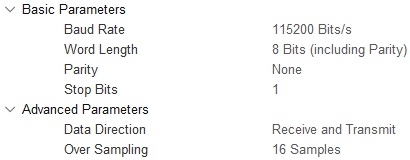
\includegraphics[width=100mm]{Rysunki/Rozdzial4/usart3_parameters.jpg}
    \caption{USART3 and USART6 configuration}
    \label{fig:my_label}
\end{figure}

The next step consists of setting up the HSE in the System Core section of the RRC tab in the BYPASS mode, similarly as in case of the Ethernet interface, in order to use the ST-Link clock signal for clocking the microcontroller.

\begin{figure}[!ht]
    \centering
    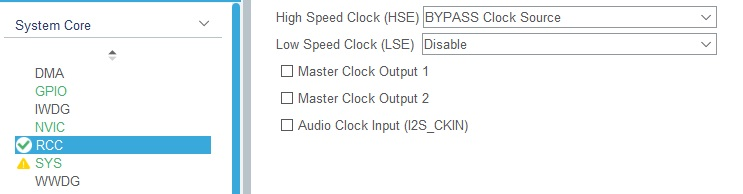
\includegraphics[width=155mm]{Rysunki/Rozdzial4/rcc_wifi.jpg}
    \caption{HSE clock setup}
    \label{fig:my_label}
\end{figure}

In the \emph{Clock Configuration} tab, the system clock frequency was set via the configurator to 180 MHz, as shown on figure 4.15.

\begin{figure}[!ht]
    \centering
    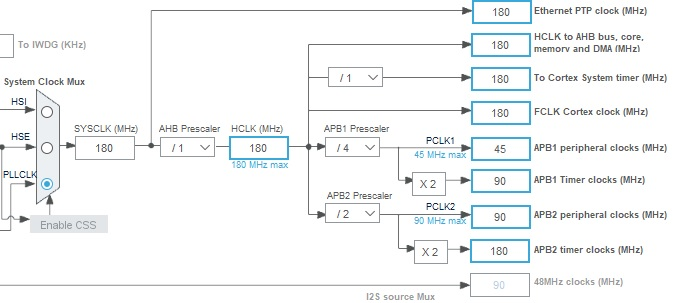
\includegraphics[width=155mm]{Rysunki/Rozdzial4/wifi_zegary.jpg}
    \caption{Target frequencies in the clock manager}
    \label{fig:my_label}
\end{figure}

The last steop of the configuration process required configuring one of the GPIO ports in the output mode, in order to control the \emph{enable} line of the Wi-Fi module. In order to activate the module and enable operating it, the line required a high logical state. Line PB3 was used for this purpose, keeping its default parameters, for which the monitoring and modification options are available in the GPIO tab of the \emph{System Core} section. They were presented on figures 4.16 and 4.17.

\begin{figure}[!ht]
    \centering
    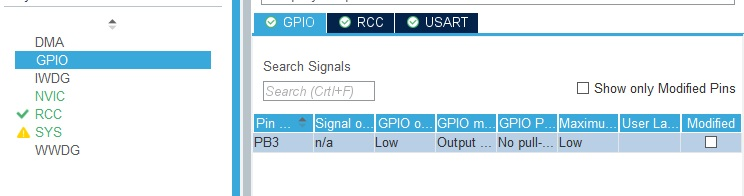
\includegraphics[width=155mm]{Rysunki/Rozdzial4/gpio_pb3.jpg}
    \caption{Configured GPIO lines}
    \label{fig:my_label}
\end{figure}

\begin{figure}[!ht]
    \centering
    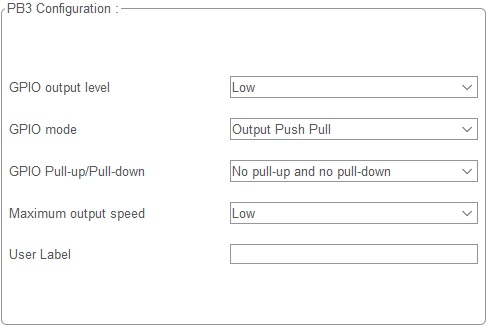
\includegraphics[width=100mm]{Rysunki/Rozdzial4/gpio_pb3_2.jpg}
    \caption{PB3 line parameters}
    \label{fig:my_label}
\end{figure}

The ESP8266 module contains a functioning implementation of the TCP/IP stack, and as such enabling the LwIP stack in the platform configurator was not required. Based on this configuration, the source was generated, which was subsequently extended with snippets that configure the Wi-Fi module and implement the echo server functionality. Listing 4.18 shows the contents of the \textit{main()} function and the globally available elements.

\cppcode{Listingi/WiFi_main.c}{\textit{main()} function and global elements}

The global elements were defined as:

\begin{itemize}
    \item [$\bullet$] character buffer for reception from the Wi-Fi module;
    \item [$\bullet$] character buffer for formatted message to be sent back;
    \item [$\bullet$] macro defining the Wi-Fi configuration commands amount;
    \item [$\bullet$] look up table containing the commands for configuring the Wi-Fi module.
\end{itemize}

The result of each of the configuration commands was described via comments inside listing 4.18. For privacy protection reasons, the password contained in the listing for the \textit{AT+CWJAP} command was censored with asterisks.

The \textit{main()} function consists of several key sections. The first one is the generated configuration section for each of the interfaces and microcontroller components, such as GPIO, system clock and USART interfaces. This section was extended with setting the PB3 line connected to the \emph{enable} input of the Wi-Fi module into high logical state.

Second section is the configuration loop. Is is tasked with performing the reset and configuration of the Wi-Fi module in a way which enables connection and two-way transmission of messages. These commands are subsequently:

\newpage

\begin{itemize}
    \item [$\bullet$] \emph{AT+RST} - module reset;
    \item [$\bullet$] \emph{ATE0} - disabling the configuration commands echo;
    \item [$\bullet$] \emph{AT} - communication test with the module;
    \item [$\bullet$] \emph{AT+GMR} - acquiring module firmware version;
    \item [$\bullet$] \emph{AT+CWMODE=1} - configuring the module into client mode;
    \item [$\bullet$] \emph{AT+CIPMODE=0} - configuring the received message format as "+IPD,\newline<channel>,<byte count>,<data>";
    \item [$\bullet$] \emph{AT+CIPMUX=1} - enabling multiconnectivity;
    \item [$\bullet$] \emph{AT+CIPSERVER=1,7} - configuring the server on port 7;
    \item [$\bullet$] \emph{AT+CWMODE=?} - verifying the operating mode;
    \item [$\bullet$] \emph{AT+CWJAP=<SSID>,<password>} - connecting to the Wi-Fi network;
    \item [$\bullet$] \emph{AT+CIPSTA?} - querrying connection status;
    \item [$\bullet$] \emph{AT+CIFSR} - acquiring the server IP address;
\end{itemize}

After sending the module reset command, the microcontroller awaits 1 second before transmitting subsequent commands. Each transmission consists of sending the command to the module, clearing the reception buffer using the \textit{clr\char`_buffer()} function presented on listing 4.19, and receiving the feedback from the module. After the \emph{AT+CWJAP} querry, the microcontroller awaits acquiring an IP address from DHCP in 1-second intervals, by querrying the connection status via the \textit{is\char`_busy()} function shown on listing 4.20. As long as the status informs that the module is busy, the process is repeated. Feedback from the module is relayed to the overseeing computer via the serial port. 

\cppcode{Listingi/clr_buffer.c}{Reception buffer clear function}

\newpage
\cppcode{Listingi/is_busy.c}{Wi-Fi module state querry function}

The third section of the \textit{main()} function contains the operating loop, which acts as the echo server functionality. Inside it, a reception buffer is cleared and data is read from the module when an event such as establishing connection or data reception occurs. In case of receiving a non-empty feedback message, the echo functionality is prepared inside the \textit{prepare\char`_echo()} function, which code can be found in listing 4.21.

\cppcode{Listingi/prepare_echo.c}{Preparing the echo functionality}

If the received feedback message starts with the "+IPD" sequence, the program extracts the number of bytes and its content in order to properly format it and prepare it for sending back. Readiness for sending is stated by the \textit{ready\char`_to\char`_send} flag. In case of extracting the message, a "send data" command is transmitted, followed by the message content in the third section of the \textit{main()} function.\ After performing the echo transmission, the \textit{ready\char`_to\char`_send} flag is reset/

%=================================================================================================
\section{Solution tests}

\subsection{Ethernet interface}

During the testing phase, following functionalities were validated:

\begin{itemize}
    \item [$\bullet$] communication with the overseeing computer via the serial port, acquiring information about the MAC address and the connection state; 
    \item [$\bullet$] exchanging the ping via Windows command prompt;
    \item [$\bullet$] connection and two-way exchange via Hercules SETUP Utility software.
\end{itemize}

Figures 4.18, 4.19 and 4.20 showcase the results of carried out tests. The first action included acquiring the IP address of the module via USART serial interface. Subsequently, the connection could be validated using the \emph{ping} command, and the echo server functionality could be verified using the Hercules SETUP Utility. All of the tests were successful, confirming the proper functioning of the Ethernet network interface. 

\begin{figure}[!ht]
    \centering
    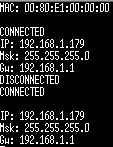
\includegraphics[width=50mm]{Rysunki/Rozdzial4/usart_ethernet.jpg}
    \caption{Serial port communication}
    \label{fig:my_label}
\end{figure}

\begin{figure}[!ht]
    \centering
    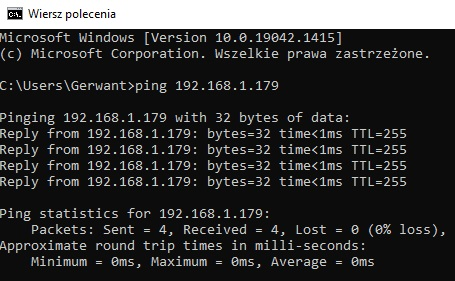
\includegraphics[width=130mm]{Rysunki/Rozdzial4/ping_ethernet.jpg}
    \caption{Verifying connection via ping}
    \label{fig:my_label}
\end{figure}

\begin{figure}[!ht]
    \centering
    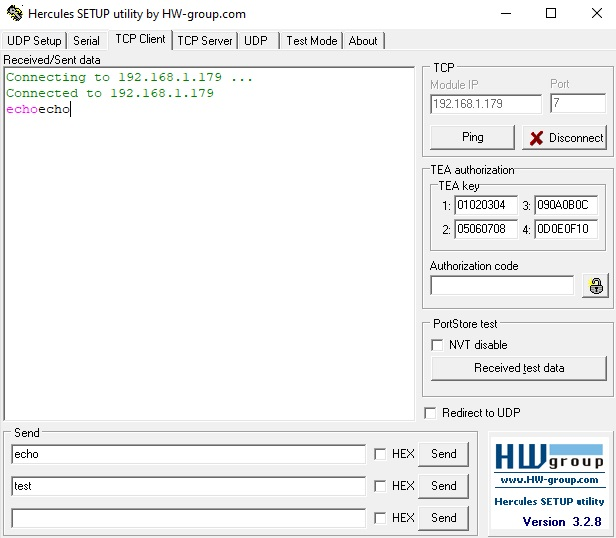
\includegraphics[width=110mm]{Rysunki/Rozdzial4/hercules_ethernet.jpg}
    \caption{Two-way communication validation using Hercules SETUP Utility}
    \label{fig:my_label}
\end{figure}

\newpage
\subsection{Wi-Fi wireless interface}

The figure 4.21 showcases a picture of the prepared circuit. Similarly to the Ethernet interface, the same set of tests was performed. Due to the reset of the device, on picture 4.22 some unreadable messages can be seen, caused by the different speed of transmission during the bootloader execution of the module. Just like in the case of the Ethernet interface, first the IP address of the module was acquired via an USART interface, which was shown on figure 4.22 and 4.23. Subsequently communication tests were carried out using the \emph{ping} command, which is shown on figure 4.24 and the echo server functionality using the Hercules SETUP Utility software shown on figure 4.25. All tests were successful.

\begin{figure}[!ht]
    \centering
    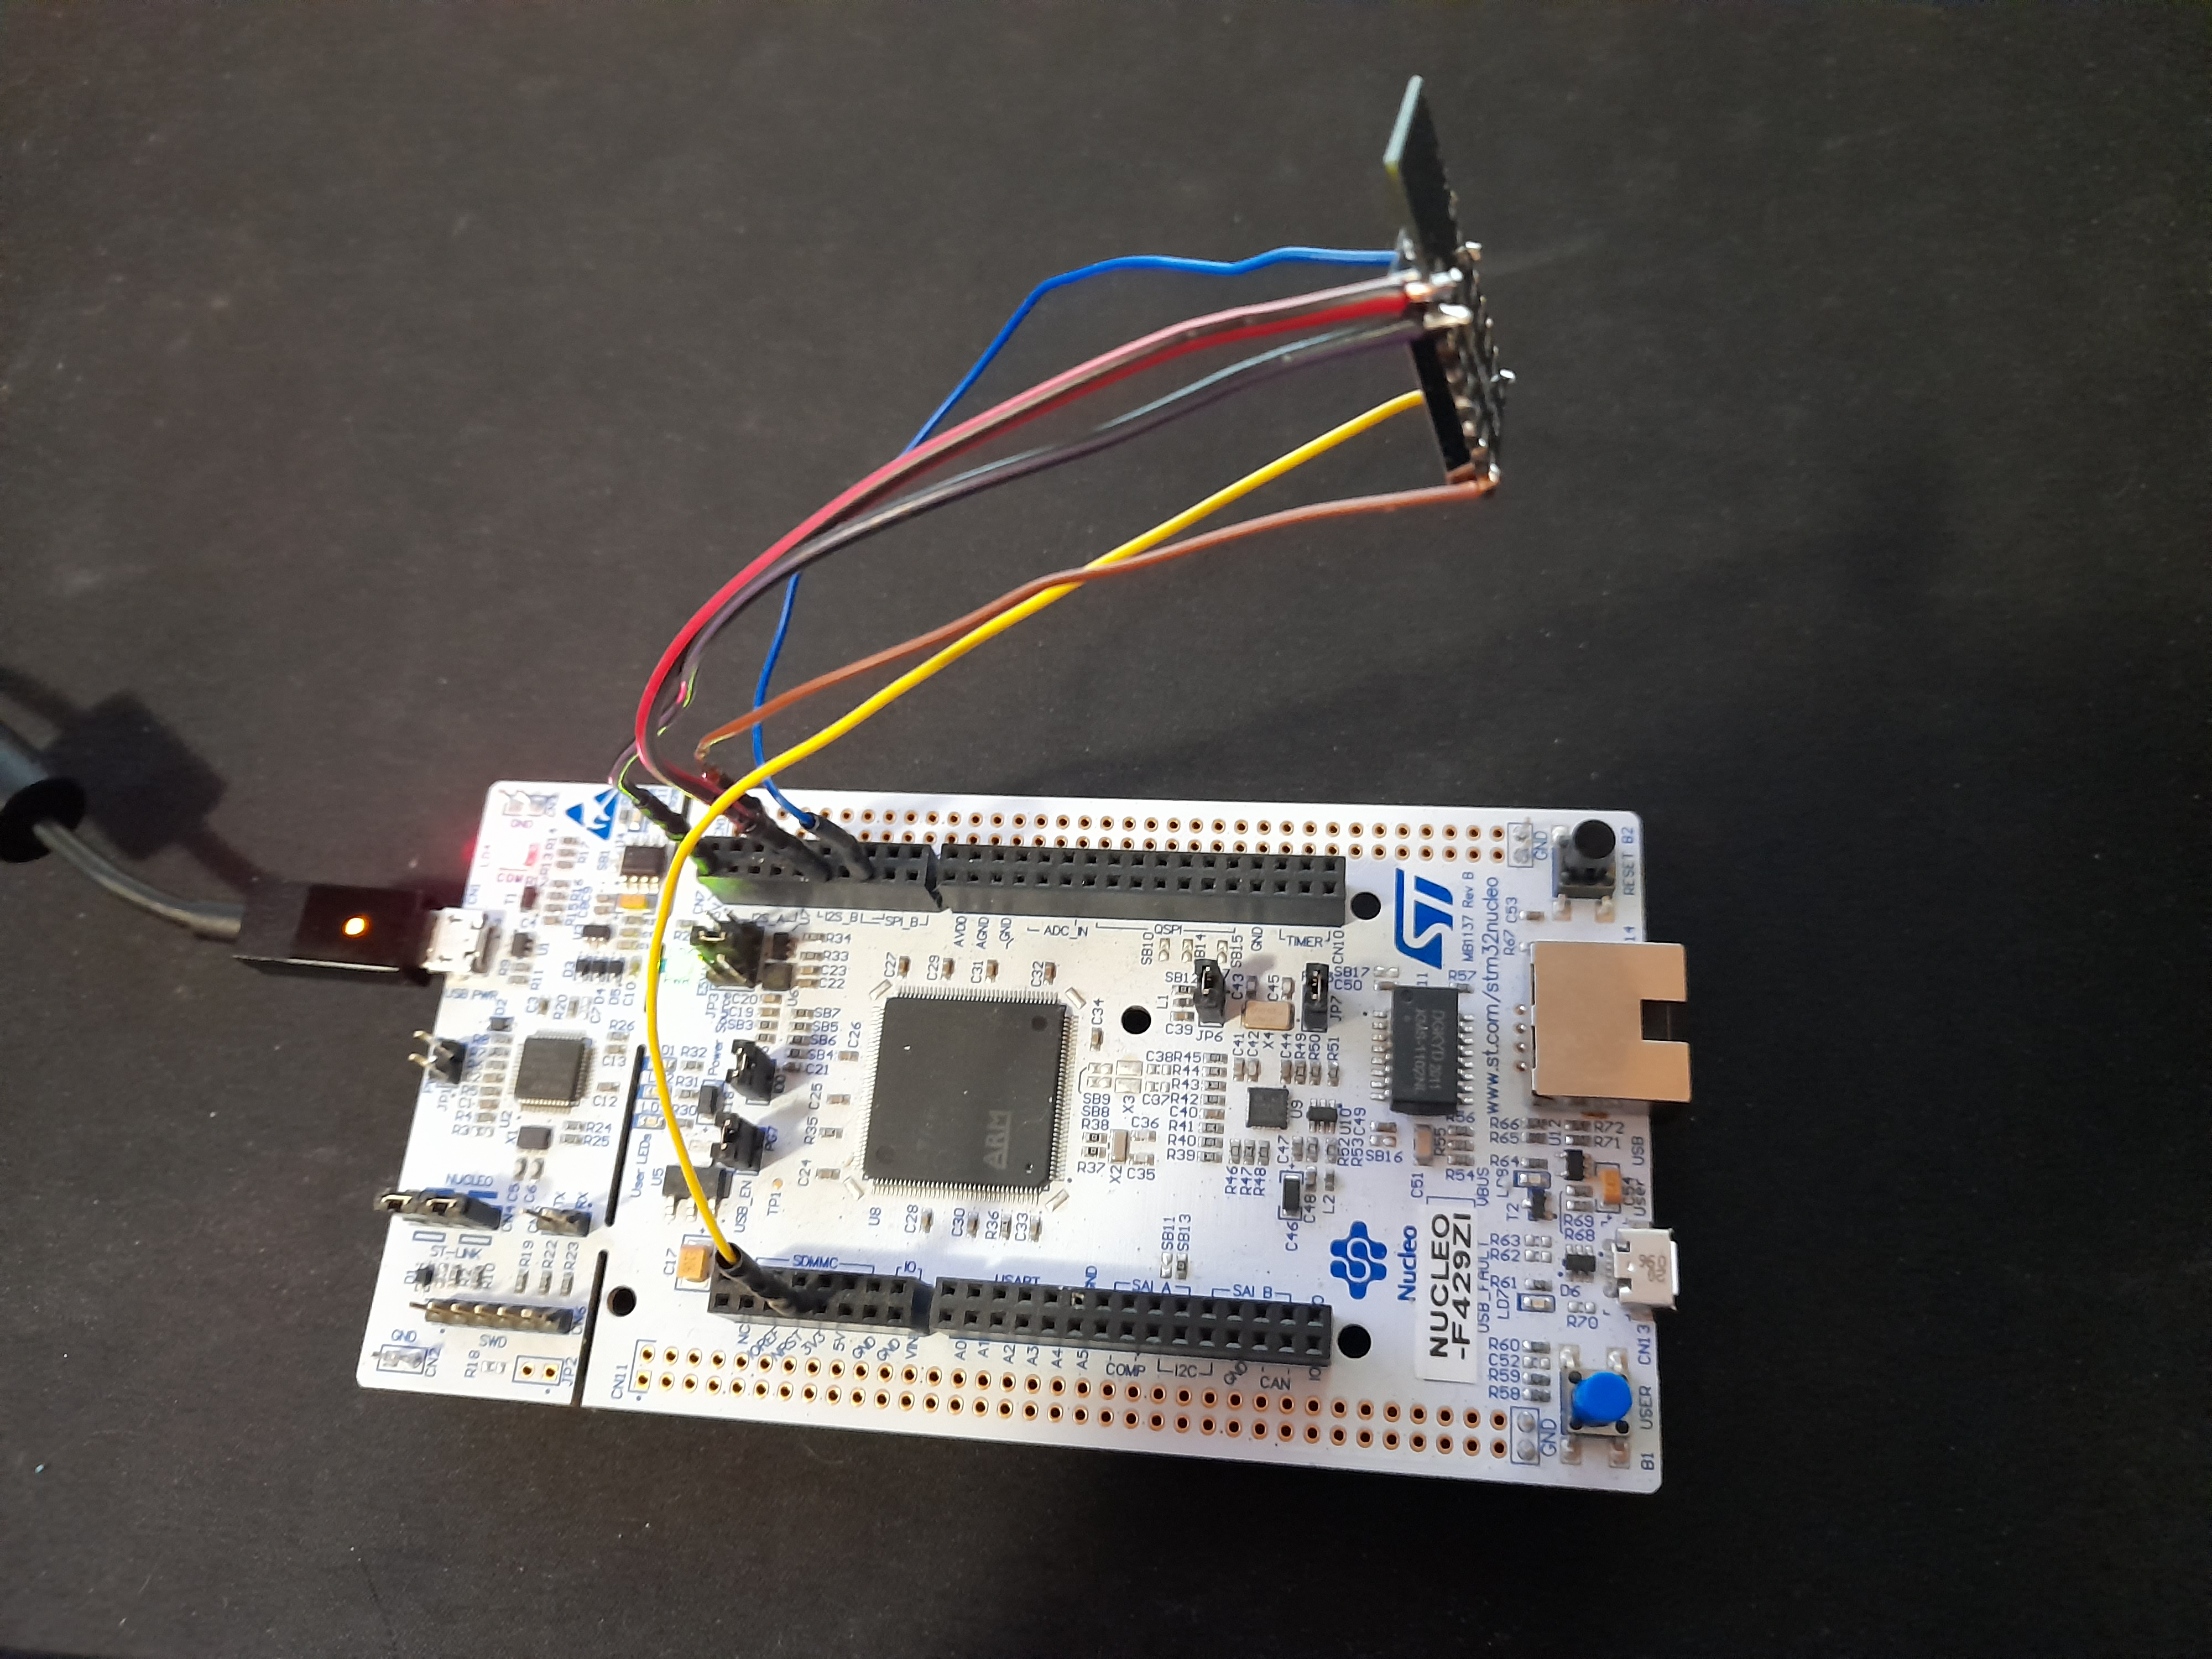
\includegraphics[width=80mm]{Rysunki/Rozdzial4/modul.jpg}
    \caption{Constructed circuit}
    \label{fig:my_label}
\end{figure}

\begin{figure}[!ht]
\begin{minipage}[b]{0.4\textwidth}
    \centering
    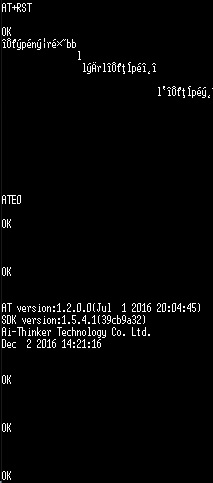
\includegraphics[width=50mm]{Rysunki/Rozdzial4/wifi_usart_1.jpg}
    \caption{Communication with overseeing computer pt. 1}
  \end{minipage}
  \hfill
  \begin{minipage}[b]{0.4\textwidth}
    \centering
    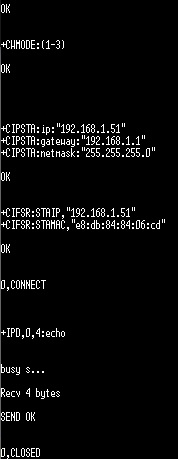
\includegraphics[width=50mm]{Rysunki/Rozdzial4/wifi_usart_2.jpg}
    \caption{Communication with overseeing computer pt. 2}
  \end{minipage}
\end{figure}


\begin{figure}[!ht]
    \centering
    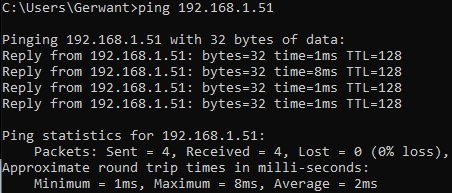
\includegraphics[width=120mm]{Rysunki/Rozdzial4/wifi_ping.jpg}
    \caption{Testing connectivity using \textit{ping}}
    \label{fig:my_label}
\end{figure}

\begin{figure}[!ht]
    \centering
    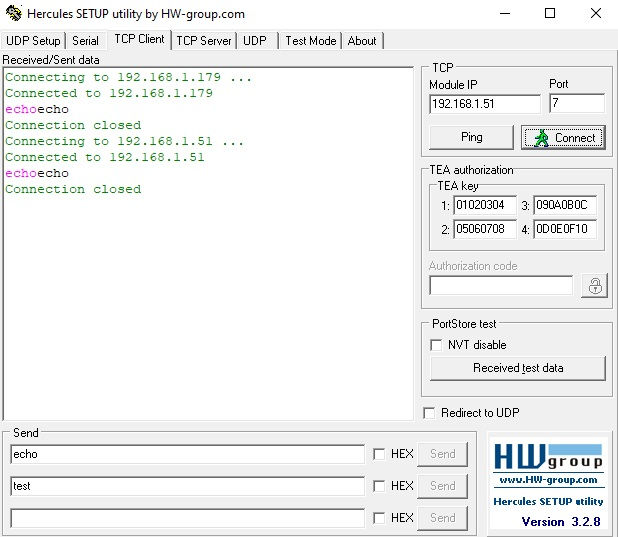
\includegraphics[width=130mm]{Rysunki/Rozdzial4/wifi_hercules.jpg}
    \caption{Two-sided communication using Hercules SETUP Utility software}
    \label{fig:my_label}
\end{figure}


\chapter{Dyskusja rezultatów i wnioski końcowe}
%=================================================================================================
W wyniku analizy istniejących rozwiązań implementacyjnych interfejsów sieciowych oraz analizy struktury stosu TCP/IP podjęte zostały decyzje o wyborze platform sprzętowych do implementacji modułu IoT w postaci serwera echo z obsługą połączeń sieciowych w części praktycznej niniejszej pracy. 

Podczas realizacji niniejszej pracy wyciągnięte zostały następujące uwagi i wnioski:

\begin{itemize}
    \item [$\bullet$] Istnieje wiele dostępnych na rynku rozwiązań implementacyjnych interfejsów sieciowych, w tym zarówno sieci przewodowych jak i bezprzewodowych;
    \item [$\bullet$] Część platform sprzętowych posiada gotowe implementacje części sprzętowej interfejsów sieciowych, jak np. wlutowane złącze 8P8C lub moduł Wi-Fi umieszczony na pokładzie płytki PCB;
    \item [$\bullet$] Istnieje kilka implementacji stosu TCP/IP różniących się od siebie kwestiami takimi jak oferowane funkcjonalności oraz zużycie pamięci i czasu przetwarzania. Przykładami implementacji stosu TCP/IP o otwartej licencji są stosy LwIP oraz uIP.
    \item [$\bullet$] Mimo zastosowania tego samej częstotliwości zegara systemowego, na podstawie obserwacji szybkości pojawiania się komunikatów w programie Hercules SETUP Utility i terminalu portu szeregowego, oraz na podstawie czasów zmierzonych przez polecenie ping, interfejs Wi-Fi charakteryzował się większym opóźnieniem przy przesyłaniu wiadomości echo niż interfejs Ethernet. W przypadku funkcjonalności echo oraz komunikacji za pomocą portu szeregowego prawdopodobną przyczyną jest konieczność komunikacji z układem mikrokontrolera za pomocą interfejsu UART oraz czas przetwarzania przez niego danych.
\end{itemize}


%========================================================================================
% Dodatki
%========================================================================================
\begin{appendix}
\appendix
	%\input{Dodatki/dodatek_a.tex}
	%\input{Dodatki/dodatek_b.tex}
\end{appendix}

%========================================================================================
% Literatura
%========================================================================================

\begin{flushleft}
	\printbibliography[title={Bibliography}]
\end{flushleft}

\end{document}
%========================================================================================
% Koniec dokumentu
%========================================================================================
